% ============================================
% MODULAÇÃO EM AMPLITUDE (AM)
% ============================================

\section{Introdução à Modulação}

\begin{frame}{Por que Modular Sinais?}

\textbf{Comunicação Banda Base} vs. \textbf{Comunicação por Portadora}

\vspace{0.2cm}

\begin{columns}[T]
\begin{column}{0.48\textwidth}
\begin{enumerate}
\item \textbf{Multiplexação (FDM):}
   Múltiplos sinais compartilham o mesmo meio, cada um em frequência diferente

\item \textbf{Propagação e Antenas:}
   Antena eficiente: tamanho $\approx \lambda/4$\\
   1 kHz: $\lambda = 300$ km (impraticável)\\
   1 MHz: $\lambda = 300$ m (antena de 75 m)
\end{enumerate}
\end{column}
\begin{column}{0.48\textwidth}
\begin{enumerate}\setcounter{enumi}{2}
\item \textbf{Largura de Banda vs. Frequência:}
   Aloca sinais em bandas apropriadas, reduz ruído e interferência

\item \textbf{Processamento de Sinal:}
   Facilita filtragem, amplificação e melhora relação sinal-ruído
\end{enumerate}
\end{column}
\end{columns}

\end{frame}

% ============================================

\begin{frame}{Ideia Central: O que é Modular?}

\begin{center}
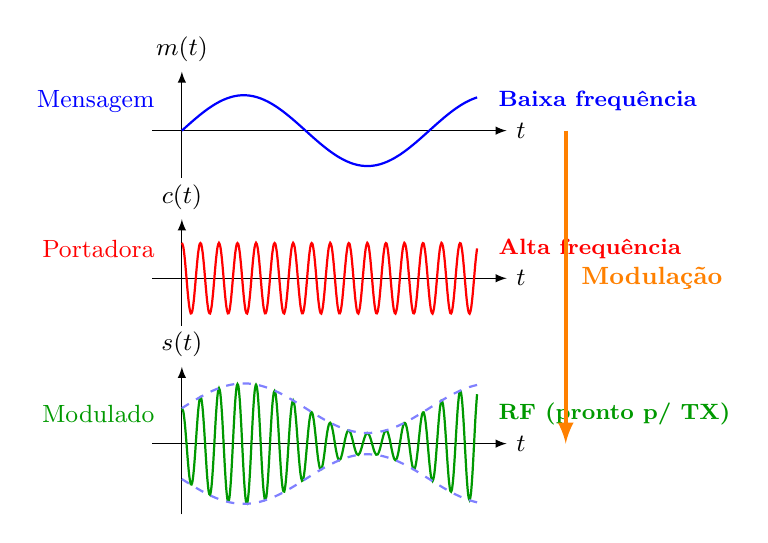
\begin{tikzpicture}[>=latex, scale=0.75]
% Sinal de mensagem
\begin{scope}[yshift=2.5cm]
\draw[->] (-0.5,0) -- (5.5,0) node[right, font=\small] {$t$};
\draw[->] (0,-0.8) -- (0,1) node[above, font=\small] {$m(t)$};
\draw[thick, blue, smooth] plot[domain=0:5, samples=80] (\x, {0.6*sin(1.5*\x r)});
\node[left, font=\small, blue] at (-0.3,0.5) {Mensagem};
\node[right, font=\footnotesize, blue] at (5.2,0.5) {\textbf{Baixa frequência}};
\end{scope}

% Portadora
\begin{scope}[yshift=0cm]
\draw[->] (-0.5,0) -- (5.5,0) node[right, font=\small] {$t$};
\draw[->] (0,-0.8) -- (0,1) node[above, font=\small] {$c(t)$};
\draw[thick, red, smooth] plot[domain=0:5, samples=200] (\x, {0.6*cos(20*\x r)});
\node[left, font=\small, red] at (-0.3,0.5) {Portadora};
\node[right, font=\footnotesize, red] at (5.2,0.5) {\textbf{Alta frequência}};
\end{scope}

% Sinal modulado
\begin{scope}[yshift=-2.8cm]
\draw[->] (-0.5,0) -- (5.5,0) node[right, font=\small] {$t$};
\draw[->] (0,-1.2) -- (0,1.3) node[above, font=\small] {$s(t)$};
\draw[thick, green!60!black, smooth] plot[domain=0:5, samples=200] (\x, {0.6*(1+0.7*sin(1.5*\x r))*cos(20*\x r)});
\draw[thick, dashed, blue!50, smooth] plot[domain=0:5, samples=80] (\x, {0.6*(1+0.7*sin(1.5*\x r))});
\draw[thick, dashed, blue!50, smooth] plot[domain=0:5, samples=80] (\x, {-0.6*(1+0.7*sin(1.5*\x r))});
\node[left, font=\small, green!60!black] at (-0.3,0.5) {Modulado};
\node[right, font=\footnotesize, green!60!black] at (5.2,0.5) {\textbf{RF (pronto p/ TX)}};
\end{scope}

% Setas indicando operação
\draw[->, ultra thick, orange] (6.5,2.5) -- (6.5,-2.8);
\node[right, font=\small, orange] at (6.6,0) {\textbf{Modulação}};
\end{tikzpicture}
\end{center}

\textbf{Modular = ``embalar'' a mensagem dentro de uma portadora de alta frequência}

\end{frame}

% ============================================

\begin{frame}{Classificação das Modulações}

\textbf{Modulação Analógica:} Parâmetro da portadora varia continuamente com mensagem

\vspace{0.3cm}

\textbf{Portadora:} $c(t) = A_c \cos(2\pi f_c t + \phi_c)$

\vspace{0.5cm}

\textbf{Três parâmetros moduláveis:}

\begin{columns}[T]
\begin{column}{0.55\textwidth}
\begin{enumerate}
\item \textbf{Amplitude} $A_c$:
   \begin{itemize}
   \item Modulação em Amplitude (AM)
   \item Variantes: DSB-SC, DSB-LC, SSB, VSB
   \end{itemize}

\item \textbf{Frequência} $f_c$:
   \begin{itemize}
   \item Modulação em Frequência (FM)
   \end{itemize}

\item \textbf{Fase} $\phi_c$:
   \begin{itemize}
   \item Modulação em Fase (PM)
   \end{itemize}
\end{enumerate}
\end{column}
\begin{column}{0.42\textwidth}
\begin{center}
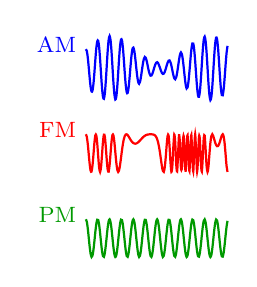
\begin{tikzpicture}[>=latex, scale=0.6]
% AM
\draw[thick, blue, smooth] plot[domain=0:3, samples=150] (\x, {(1+0.7*sin(3*\x r))*0.4*cos(25*\x r)});
\node[left, font=\footnotesize, blue] at (0,0.5) {AM};
% FM
\begin{scope}[yshift=-1.8cm]
\draw[thick, red, smooth] plot[domain=0:3, samples=150] (\x, {0.4*cos((25+8*sin(3*\x r))*\x r)});
\node[left, font=\footnotesize, red] at (0,0.5) {FM};
\end{scope}
% PM
\begin{scope}[yshift=-3.6cm]
\draw[thick, green!60!black, smooth] plot[domain=0:3, samples=150] (\x, {0.4*cos(25*\x r + 2*sin(3*\x r))});
\node[left, font=\footnotesize, green!60!black] at (0,0.5) {PM};
\end{scope}
\end{tikzpicture}
\end{center}
\end{column}
\end{columns}

\vspace{0.3cm}

%\textbf{Nesta aula:} Modulação em Amplitude e suas variantes

\end{frame}

% ============================================

\begin{frame}{Diagrama de Blocos: Sistema de Comunicação}

\begin{center}
\begin{tikzpicture}[>=latex, scale=0.75,
    bloco/.style={draw, rectangle, rounded corners=3pt, minimum width=1.8cm, minimum height=0.8cm, font=\footnotesize}]
% Transmissor
\node[bloco, fill=blue!15] (mod) at (0,0) {Modulador};
\node[bloco, fill=blue!8] (tx) at (3,0) {Transmissor};

% Canal
\node[bloco, fill=yellow!20] (canal) at (6,0) {Canal};

% Receptor
\node[bloco, fill=green!8] (rx) at (9,0) {Receptor};
\node[bloco, fill=green!15] (demod) at (12,0) {Demodulador};

% Conexões
\draw[->] (-2,0) -- node[above, font=\small] {$m(t)$} (mod.west);
\draw[->] (mod.east) -- node[above, font=\footnotesize] {$s(t)$} (tx.west);
\draw[->] (tx.east) -- (canal.west);
\draw[->] (canal.east) -- (rx.west);
\draw[->] (rx.east) -- node[above, font=\footnotesize] {$r(t)$} (demod.west);
\draw[->] (demod.east) -- node[above, font=\small] {$\hat{m}(t)$} (14,0);

% Portadora
\draw[->] (mod.south) -- ++(0,-1.0) node[below, font=\footnotesize] {$A_c\cos(2\pi f_c t)$};
\draw[->] (demod.south) -- ++(0,-1.0) node[below, font=\footnotesize] {$\cos(2\pi f_c t)$};

% Labels acima
\node[above=0.4cm of mod, font=\footnotesize] {Mensagem};
\node[above=0.4cm of tx, font=\footnotesize] {RF};
\node[above=0.4cm of rx, font=\footnotesize] {RF};
\node[above=0.4cm of demod, font=\footnotesize] {Mensagem};
\end{tikzpicture}
\end{center}

\textbf{Componentes principais:}
\begin{itemize}
\item \textbf{Modulador:} Combina mensagem $m(t)$ com portadora
\item \textbf{Canal:} Meio de transmissão (ar, cabo, fibra)
\item \textbf{Demodulador:} Recupera $m(t)$ do sinal modulado
\end{itemize}

\end{frame}

% ============================================

\section{AM DSB-SC}

% ============================================
% SLIDE: Definição DSB-SC
% ============================================
\begin{frame}{AM DSB-SC: Double Sideband Suppressed Carrier}

\begin{columns}[T]
\begin{column}{0.48\textwidth}

\begin{block}{Definição}
\vspace{-0.3cm}
\[
s(t) = A_c\, m(t) \cos(2\pi f_c t)
\]
\end{block}

\onslide<2->{
\begin{itemize}
\item $m(t)$: mensagem (banda $W$)
\item $A_c$: amplitude da portadora
\item $f_c \gg W$
\end{itemize}
}

\onslide<3->{
\vspace{0.2cm}
\textbf{Características:}
\begin{itemize}
\item Portadora \textbf{suprimida}
\item Simples: um multiplicador
\item Requer detecção \textbf{coerente}
\end{itemize}
}

\end{column}
\begin{column}{0.50\textwidth}
\onslide<2->{
\begin{center}
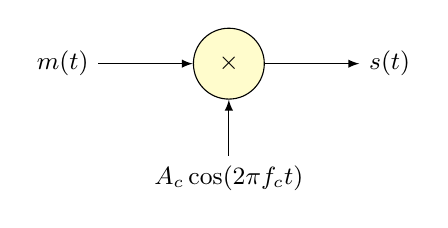
\begin{tikzpicture}[>=latex, scale=0.6]
% Modulador bloco
\node[draw, circle, fill=yellow!20, minimum size=0.9cm, font=\small] (mult) at (0,0) {$\times$};
\draw[<-] (mult.west) -- ++(-2,0) node[left, font=\small] {$m(t)$};
\draw[<-] (mult.south) -- ++(0,-1.2) node[below, font=\small] {$A_c\cos(2\pi f_c t)$};
\draw[->] (mult.east) -- ++(2,0) node[right, font=\small] {$s(t)$};
\end{tikzpicture}
\end{center}
}

\onslide<3->{
\vspace{-0.2cm}
\begin{center}
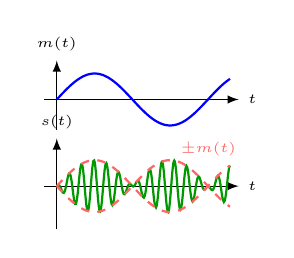
\begin{tikzpicture}[>=latex, scale=0.55]
% m(t)
\draw[->] (-0.3,0) -- (4.2,0) node[right, font=\tiny] {$t$};
\draw[->] (0,-0.7) -- (0,0.9) node[above, font=\tiny] {$m(t)$};
\draw[thick, blue, smooth] plot[domain=0:4, samples=80] (\x, {0.6*sin(1.8*\x r)});
% s(t)
\begin{scope}[yshift=-2cm]
\draw[->] (-0.3,0) -- (4.2,0) node[right, font=\tiny] {$t$};
\draw[->] (0,-1) -- (0,1.1) node[above, font=\tiny] {$s(t)$};
\draw[thick, green!60!black, smooth] plot[domain=0:4, samples=200]
  (\x, {0.6*sin(1.8*\x r)*cos(22*\x r)});
\draw[thick, dashed, red!60, smooth] plot[domain=0:4, samples=80]
  (\x, {0.6*sin(1.8*\x r)});
\draw[thick, dashed, red!60, smooth] plot[domain=0:4, samples=80]
  (\x, {-0.6*sin(1.8*\x r)});
\node[font=\tiny, red!60] at (3.5,0.85) {$\pm m(t)$};
\end{scope}
\end{tikzpicture}
\end{center}
}
\end{column}
\end{columns}

\end{frame}

% ============================================
% SLIDE: Visualização tempo DSB-SC (figuras geradas)
% ============================================
\begin{frame}{Visualização DSB-SC no Tempo e na Frequência}

\begin{center}
\only<1>{
\includegraphics[width=\figFull, trim=0 220bp 0 0, clip]{figures/cap4/am_dsb_sc.pdf}

\vspace{0.3cm}
\textbf{Mensagem} $m(t)$ e \textbf{portadora} $c(t)$: sinais de entrada do modulador
}
\only<2>{
\includegraphics[width=\figFull, trim=0 0 0 440bp, clip]{figures/cap4/am_dsb_sc.pdf}

\vspace{0.3cm}
\textbf{Sinal modulado} $s(t)$: envelope segue $|m(t)|$ com \textbf{inversão de fase} quando $m(t) < 0$
}
\end{center}

\end{frame}

% ============================================
% SLIDE: Análise Espectral — derivação com overlays
% ============================================
\begin{frame}{Análise Espectral do DSB-SC}

\only<1>{
$s(t) = A_c m(t) \cos(2\pi f_c t)$

\vspace{0.5cm}

Usando $\cos(2\pi f_c t) = \dfrac{e^{j2\pi f_c t} + e^{-j2\pi f_c t}}{2}$:
\[
s(t) = A_c m(t) \frac{e^{j2\pi f_c t} + e^{-j2\pi f_c t}}{2}
\]
}

\only<2>{
Pela propriedade de deslocamento em frequência:
\[
m(t)e^{j2\pi f_c t} \xleftrightarrow{\mathcal{F}} M(f - f_c)
\]

Aplicando aos dois termos:

\vspace{-0.2cm}
\[
A_c m(t) \frac{e^{j2\pi f_c t}}{2} \xleftrightarrow{\mathcal{F}} \frac{A_c}{2}M(f - f_c)
\]
\[
A_c m(t) \frac{e^{-j2\pi f_c t}}{2} \xleftrightarrow{\mathcal{F}} \frac{A_c}{2}M(f + f_c)
\]
}

\only<3>{
\textbf{Resultado:}

\[
\boxed{S(f) = \frac{A_c}{2}\bigl[M(f - f_c) + M(f + f_c)\bigr]}
\]

\vspace{0.3cm}

\begin{center}
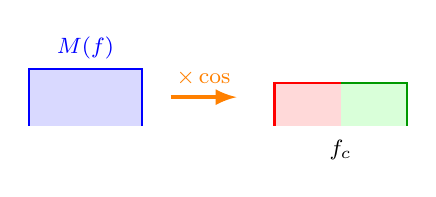
\begin{tikzpicture}[>=latex, scale=0.6]
% M(f) original
\fill[blue!15] (-1.2,0) -- (-1.2,1.2) -- (1.2,1.2) -- (1.2,0) -- cycle;
\draw[thick, blue] (-1.2,0) -- (-1.2,1.2) -- (1.2,1.2) -- (1.2,0);
\node[above, font=\footnotesize, blue] at (0,1.2) {$M(f)$};
% Seta
\draw[->, ultra thick, orange] (1.8,0.6) -- (3.2,0.6)
  node[midway, above, font=\footnotesize] {$\times\cos$};
% Cópia em +fc
\fill[red!15] (4,0) -- (4,0.9) -- (5.4,0.9) -- (5.4,0) -- cycle;
\fill[green!15] (5.4,0) -- (5.4,0.9) -- (6.8,0.9) -- (6.8,0) -- cycle;
\draw[thick, red] (4,0) -- (4,0.9) -- (5.4,0.9);
\draw[thick, green!60!black] (5.4,0.9) -- (6.8,0.9) -- (6.8,0);
\node[below, font=\footnotesize] at (5.4,-0.1) {$f_c$};
\end{tikzpicture}
\end{center}

\textbf{Espectro de $m(t)$ ``copiado'' para $\pm f_c$}
}

\end{frame}

% ============================================
% SLIDE: Visualização espectral progressiva
% ============================================
\begin{frame}{O que Acontece no Espectro?}

% --- Overlays 1--2: M(f) e C(f) ---
\only<1-2>{
\begin{center}
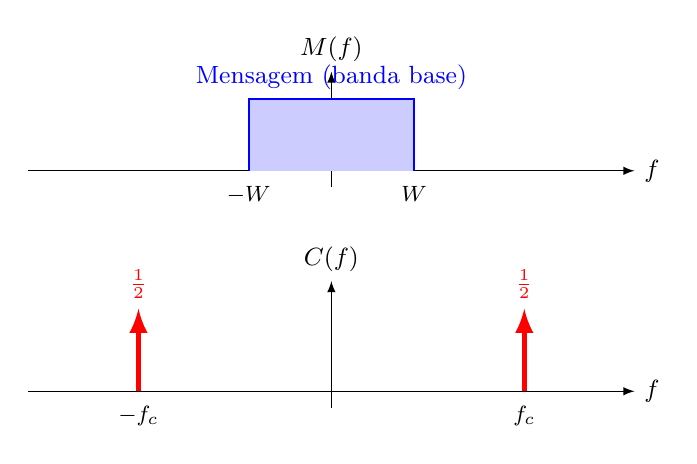
\begin{tikzpicture}[>=latex, scale=0.7]

% M(f) na banda base
\begin{scope}[yshift=2cm]
\draw[->] (-5.5,0) -- (5.5,0) node[right, font=\small] {$f$};
\draw[->] (0,-0.3) -- (0,1.8) node[above, font=\small] {$M(f)$};
\fill[blue!20] (-1.5,0) -- (-1.5,1.3) -- (1.5,1.3) -- (1.5,0) -- cycle;
\draw[thick, blue] (-1.5,0) -- (-1.5,1.3) -- (1.5,1.3) -- (1.5,0);
\node[below, font=\footnotesize] at (-1.5,-0.1) {$-W$};
\node[below, font=\footnotesize] at (1.5,-0.1) {$W$};
\node[above, font=\small, blue] at (0,1.3) {Mensagem (banda base)};
\end{scope}

% C(f) — espectro do cosseno
\onslide<2->{
\begin{scope}[yshift=-2cm]
\draw[->] (-5.5,0) -- (5.5,0) node[right, font=\small] {$f$};
\draw[->] (0,-0.3) -- (0,2) node[above, font=\small] {$C(f)$};
% Delta em +fc
\draw[thick, red, ->, line width=2pt] (3.5,0) -- (3.5,1.5);
\node[above, font=\small, red] at (3.5,1.5) {$\frac{1}{2}$};
\node[below, font=\footnotesize] at (3.5,-0.1) {$f_c$};
% Delta em -fc
\draw[thick, red, ->, line width=2pt] (-3.5,0) -- (-3.5,1.5);
\node[above, font=\small, red] at (-3.5,1.5) {$\frac{1}{2}$};
\node[below, font=\footnotesize] at (-3.5,-0.1) {$-f_c$};
\end{scope}
}

\end{tikzpicture}
\end{center}

\onslide<2->{
\[
\cos(2\pi f_c t) \xleftrightarrow{\mathcal{F}} \tfrac{1}{2}[\delta(f - f_c) + \delta(f + f_c)]
\]

\centering Multiplicação no tempo $=$ \textbf{convolução na frequência}: $S(f) = M(f) \ast C(f)$
}
}

% --- Overlay 3--4: Resultado S(f) ---
\only<3->{
\begin{center}

$S(f) = M(f) \ast C(f) = \dfrac{A_c}{2}[M(f - f_c) + M(f + f_c)]$

\vspace{0.3cm}

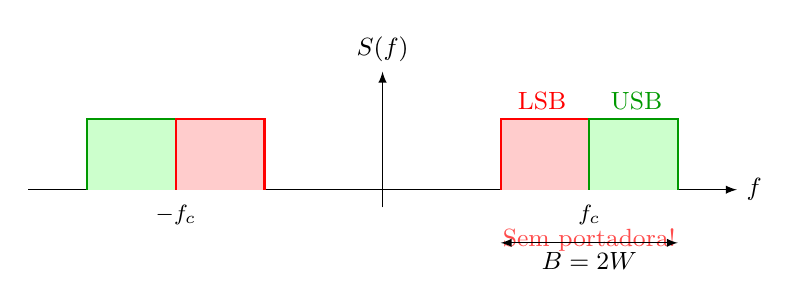
\begin{tikzpicture}[>=latex, scale=0.75]
\draw[->] (-6,0) -- (6,0) node[right, font=\small] {$f$};
\draw[->] (0,-0.3) -- (0,2) node[above, font=\small] {$S(f)$};
% LSB e USB em +fc
\fill[red!20] (2,0) -- (2,1.2) -- (3.5,1.2) -- (3.5,0) -- cycle;
\fill[green!20] (3.5,0) -- (3.5,1.2) -- (5,1.2) -- (5,0) -- cycle;
\draw[thick, red] (2,0) -- (2,1.2) -- (3.5,1.2) -- (3.5,0);
\draw[thick, green!60!black] (3.5,0) -- (3.5,1.2) -- (5,1.2) -- (5,0);
\node[above, font=\small, red] at (2.7,1.2) {LSB};
\node[above, font=\small, green!60!black] at (4.3,1.2) {USB};
% LSB e USB em -fc
\fill[green!20] (-5,0) -- (-5,1.2) -- (-3.5,1.2) -- (-3.5,0) -- cycle;
\fill[red!20] (-3.5,0) -- (-3.5,1.2) -- (-2,1.2) -- (-2,0) -- cycle;
\draw[thick, green!60!black] (-5,0) -- (-5,1.2) -- (-3.5,1.2) -- (-3.5,0);
\draw[thick, red] (-3.5,0) -- (-3.5,1.2) -- (-2,1.2) -- (-2,0);
% Labels
\node[below, font=\footnotesize] at (3.5,-0.1) {$f_c$};
\node[below, font=\footnotesize] at (-3.5,-0.1) {$-f_c$};
% Sem portadora
\onslide<4->{
\node[below, font=\small, red!70] at (3.5,-0.5) {Sem portadora!};
\draw[<->] (2,-0.9) -- (5,-0.9) node[midway, below, font=\small] {$B = 2W$};
}
\end{tikzpicture}
\end{center}
}

\end{frame}

% ============================================
% SLIDE: Largura de banda e potência
% ============================================
\begin{frame}{Largura de Banda e Potência do DSB-SC}

\begin{columns}[T]
\begin{column}{0.48\textwidth}

\textbf{Largura de banda:}
\vspace{-0.3cm}
\[
\boxed{B_{\text{DSB}} = 2W}
\]

\onslide<2->{
\vspace{-0.4cm}
\textbf{Potência transmitida:}

\vspace{-0.1cm}
Usando $\langle \cos^2(2\pi f_c t) \rangle = 1/2$:
\vspace{-0.3cm}
\[
\boxed{P_s = \frac{A_c^2 P_m}{2}}
\]
}

\onslide<3->{
\vspace{-0.4cm}
\begin{itemize}\setlength{\itemsep}{0pt}
\item Toda potência nas bandas laterais
\item Ambas bandas: \textbf{mesma informação}
\end{itemize}
}

\end{column}
\begin{column}{0.50\textwidth}
\onslide<3->{
\begin{center}
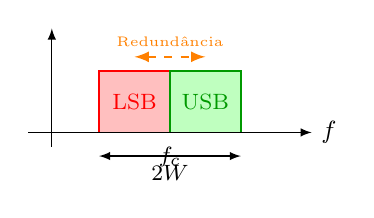
\begin{tikzpicture}[>=latex, scale=0.6]
\draw[->] (-0.5,0) -- (5.5,0) node[right, font=\small] {$f$};
\draw[->] (0,-0.3) -- (0,2.2);
% LSB
\fill[red!25] (1,0) -- (1,1.3) -- (2.5,1.3) -- (2.5,0) -- cycle;
\draw[thick, red] (1,0) -- (1,1.3) -- (2.5,1.3) -- (2.5,0);
\node[font=\footnotesize, red] at (1.75,0.65) {LSB};
% USB
\fill[green!25] (2.5,0) -- (2.5,1.3) -- (4,1.3) -- (4,0) -- cycle;
\draw[thick, green!60!black] (2.5,0) -- (2.5,1.3) -- (4,1.3) -- (4,0);
\node[font=\footnotesize, green!60!black] at (3.25,0.65) {USB};
% fc
\node[below, font=\footnotesize] at (2.5,-0.1) {$f_c$};
% Banda
\draw[<->] (1,-0.5) -- (4,-0.5) node[midway, below, font=\footnotesize] {$2W$};
% Setas indicando redundância
\draw[<->, thick, orange, dashed] (1.75,1.6) -- (3.25,1.6)
  node[midway, above, font=\tiny] {Redundância};
\end{tikzpicture}
\end{center}
}
\end{column}
\end{columns}

\end{frame}

% ============================================
% SLIDE: DSB-SC como sinal banda passante (I/Q)
% ============================================
\begin{frame}{DSB-SC é um Sinal Banda Passante}

O espectro $S(f) = \frac{A_c}{2}[M(f-f_c) + M(f+f_c)]$ mostra: a energia está em torno de $\pm f_c$, \textbf{não na origem}.

\vspace{0.2cm}

\onslide<2->{
Lembrando a representação I/Q de um sinal banda passante:
\vspace{-0.2cm}
\[
s(t) = \underbrace{s_I(t)}_{\text{em fase}}\cos(2\pi f_c t) - \underbrace{s_Q(t)}_{\text{quadratura}}\sin(2\pi f_c t)
\]
}

\onslide<3->{
\vspace{-0.2cm}
Comparando com $s(t) = A_c\,m(t)\cos(2\pi f_c t)$, identificamos:
\vspace{-0.2cm}
\[
\boxed{s_I(t) = A_c\,m(t), \qquad s_Q(t) = 0}
\]

\vspace{-0.1cm}
O DSB-SC modula \textbf{apenas a componente em fase}. A quadratura é nula!
}

\end{frame}

% ============================================
% SLIDE: Interpretação I/Q do DSB-SC
% ============================================
\begin{frame}{Interpretação no Plano I/Q}

\begin{columns}[c]
\begin{column}{0.45\textwidth}

Com $s_Q(t) = 0$, o envelope complexo é \textbf{puramente real}:
\[
\tilde{s}(t) = A_c\,m(t)
\]

\onslide<2->{
\vspace{0.2cm}
No plano I/Q, o fasor varia \textbf{apenas ao longo do eixo $I$}:

\begin{itemize}\setlength{\itemsep}{2pt}
\item Amplitude $\to$ informação
\item Fase $\to$ fixa (0 ou $\pi$)
\end{itemize}
}

\onslide<3->{
\vspace{0.2cm}
\colorbox{yellow!20}{\parbox{0.93\columnwidth}{\small\centering
Toda informação está na \textbf{amplitude} da portadora --- a \textbf{fase} não é explorada.
}}
}

\end{column}
\begin{column}{0.50\textwidth}
\begin{center}
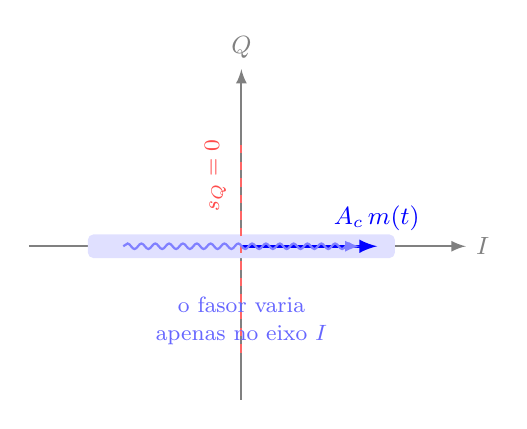
\begin{tikzpicture}[scale=1.5, >=latex]
% Axes
\draw[->, thick, gray] (-1.8,0) -- (1.9,0) node[right, font=\small] {$I$};
\draw[->, thick, gray] (0,-1.3) -- (0,1.5) node[above, font=\small] {$Q$};

% Shaded region on I axis showing m(t) range
\fill[blue!12, rounded corners=2pt] (-1.3,-0.1) rectangle (1.3,0.1);

% Vector on I axis
\draw[->, very thick, blue] (0,0) -- (1.15,0);
\node[blue, font=\small, above right] at (0.7,0.05) {$A_c\,m(t)$};

% Q = 0 annotation
\draw[dashed, red!60, thick] (0,-0.9) -- (0,0.9);
\node[red!70, font=\footnotesize, rotate=90] at (-0.22,0.6) {$s_Q = 0$};

% Oscillation arrow
\draw[->, thick, blue!50, decorate, decoration={snake, amplitude=1pt, segment length=5pt}]
  (-1.0,0) -- (1.0,0);
\node[font=\footnotesize, text=blue!60] at (0,-0.5) {o fasor varia};
\node[font=\footnotesize, text=blue!60] at (0,-0.75) {apenas no eixo $I$};

\end{tikzpicture}
\end{center}
\end{column}
\end{columns}

\end{frame}

% ============================================
% SLIDE: Exemplo DSB-SC — Enunciado
% ============================================
\begin{frame}{Exemplo: Transmissor de Rádio DSB-SC}

\begin{block}{Enunciado}
Uma estação de rádio experimental usa modulação DSB-SC para transmitir
um tom de teste de $f_m = 5\,\text{kHz}$. A portadora tem frequência
$f_c = 500\,\text{kHz}$ e amplitude $A_c = 10\,\text{V}$.
\end{block}

\begin{columns}[T]
\begin{column}{0.55\textwidth}
\onslide<2->{
\textbf{Determine:}
\begin{enumerate}
\item Expressão de $s(t)$
\item Frequências no espectro
\item Potência total transmitida
\item Largura de banda ocupada
\end{enumerate}
}
\end{column}
\begin{column}{0.43\textwidth}
\onslide<2->{
\begin{center}
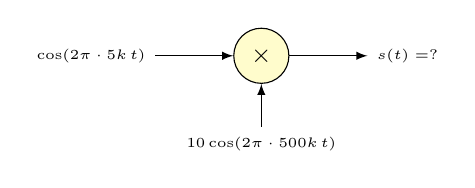
\begin{tikzpicture}[>=latex, scale=0.55]
\node[draw, circle, fill=yellow!20, minimum size=0.7cm, font=\small] (mult) at (0,0) {$\times$};
\draw[<-] (mult.west) -- ++(-1.8,0) node[left, font=\tiny] {$\cos(2\pi \cdot 5\text{k}\, t)$};
\draw[<-] (mult.south) -- ++(0,-1) node[below, font=\tiny] {$10\cos(2\pi \cdot 500\text{k}\, t)$};
\draw[->] (mult.east) -- ++(1.8,0) node[right, font=\tiny] {$s(t) = ?$};
\end{tikzpicture}
\end{center}
}
\end{column}
\end{columns}

\end{frame}

% ============================================
% SLIDE: Exemplo DSB-SC — Resolução animada
% ============================================
\begin{frame}{Resolução: Transmissor DSB-SC}

\only<1>{
\textbf{Passo 1: Expressão do sinal modulado}

\[
s(t) = A_c \cos(2\pi f_m t) \cos(2\pi f_c t) = 10\cos(2\pi \cdot 5000\, t)\cos(2\pi \cdot 500000\, t)
\]

Usando $\cos A \cos B = \frac{1}{2}[\cos(A-B) + \cos(A+B)]$:

\[
\boxed{s(t) = 5\cos(2\pi \cdot 495000\, t) + 5\cos(2\pi \cdot 505000\, t)}
\]

\begin{center}
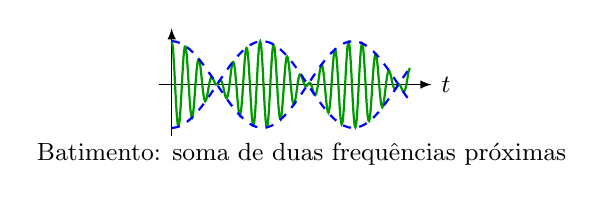
\begin{tikzpicture}[>=latex, scale=0.55]
\draw[->] (-0.3,0) -- (6,0) node[right, font=\small] {$t$};
\draw[->] (0,-1.2) -- (0,1.3);
\draw[thick, green!60!black, smooth] plot[domain=0:5.5, samples=200]
  (\x, {cos(1.5*\x r)*cos(20*\x r)});
\draw[thick, dashed, blue, smooth] plot[domain=0:5.5, samples=80]
  (\x, {cos(1.5*\x r)});
\draw[thick, dashed, blue, smooth] plot[domain=0:5.5, samples=80]
  (\x, {-cos(1.5*\x r)});
\node[font=\small] at (3,-1.6) {Batimento: soma de duas frequências próximas};
\end{tikzpicture}
\end{center}
}

\only<2>{
\textbf{Passo 2: Frequências no espectro}

\vspace{0.2cm}

\begin{columns}[T]
\begin{column}{0.45\textwidth}
\begin{itemize}
\item LSB: $f_c - f_m = 495\,\text{kHz}$
\item USB: $f_c + f_m = 505\,\text{kHz}$
\item Em $f_c = 500\,\text{kHz}$: \textbf{nada!}
\end{itemize}

\vspace{0.3cm}

\textbf{Passo 3: Potência}
\[
P_s = \frac{A_c^2}{4} = \frac{100}{4} = \boxed{25\,\text{W}}
\]

\textbf{Passo 4: Largura de banda}
\[
B = 2f_m = 2 \times 5 = \boxed{10\,\text{kHz}}
\]
\end{column}
\begin{column}{0.53\textwidth}
\begin{center}
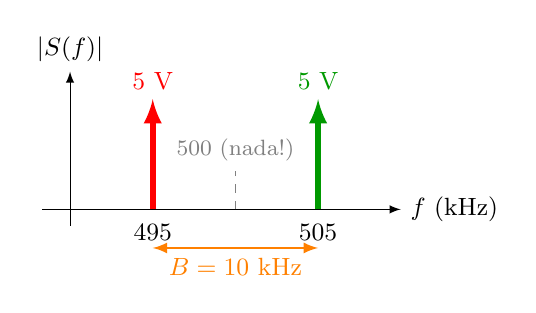
\begin{tikzpicture}[>=latex, scale=0.7]
\draw[->] (-0.5,0) -- (6,0) node[right, font=\small] {$f$ (kHz)};
\draw[->] (0,-0.3) -- (0,2.5) node[above, font=\small] {$|S(f)|$};
% LSB
\draw[thick, red, ->, line width=2pt] (1.5,0) -- (1.5,2);
\node[above, font=\small, red] at (1.5,2) {$5$ V};
\node[below, font=\small] at (1.5,-0.1) {$495$};
% USB
\draw[thick, green!60!black, ->, line width=2pt] (4.5,0) -- (4.5,2);
\node[above, font=\small, green!60!black] at (4.5,2) {$5$ V};
\node[below, font=\small] at (4.5,-0.1) {$505$};
% fc
\draw[dashed, gray] (3,0) -- (3,0.7);
\node[above, font=\footnotesize, gray] at (3,0.7) {$500$ (nada!)};
% Banda
\draw[<->, thick, orange] (1.5,-0.7) -- (4.5,-0.7)
  node[midway, below, font=\small] {$B = 10$ kHz};
\end{tikzpicture}
\end{center}
\end{column}
\end{columns}
}

\end{frame}

% ============================================
% SLIDE: Demodulação via Envelope Complexo — passo 1
% ============================================
\begin{frame}{Demodulação DSB-SC: Abordagem via Envelope Complexo}

\only<1>{
Vimos que o DSB-SC tem envelope complexo $\tilde{s}(t) = A_c\,m(t)$. Como recuperar $m(t)$?

\vspace{0.5cm}

\textbf{Receita do Módulo anterior} (passante $\to$ banda básica):

\vspace{0.3cm}

\begin{center}
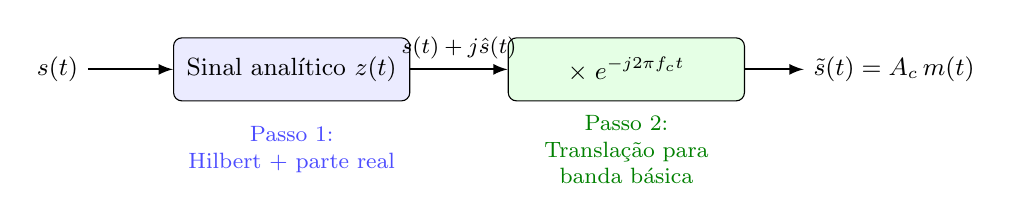
\begin{tikzpicture}[>=latex, scale=0.85,
    bloco/.style={draw, rectangle, rounded corners=3pt, minimum height=0.8cm, font=\small, fill=blue!8}]

% s(t) input
\node[font=\small] (in) at (-5,0) {$s(t)$};

% Step 1: form analytic signal
\node[bloco, minimum width=3cm] (hilb) at (-1.5,0) {Sinal analítico $z(t)$};
\draw[->, thick] (in) -- (hilb);

% Step 2: derotate
\node[bloco, minimum width=3cm, fill=green!10] (derot) at (3.5,0) {$\times\; e^{-j2\pi f_c t}$};
\draw[->, thick] (hilb) -- node[above, font=\footnotesize] {$s(t) + j\hat{s}(t)$} (derot);

% Step 3: output
\node[font=\small] (out) at (7.5,0) {$\tilde{s}(t) = A_c\,m(t)$};
\draw[->, thick] (derot) -- (out);

% Labels below
\node[font=\footnotesize, blue!70, align=center] at (-1.5,-1.2) {Passo 1:\\Hilbert + parte real};
\node[font=\footnotesize, green!50!black, align=center] at (3.5,-1.2) {Passo 2:\\Translação para\\banda básica};

\end{tikzpicture}
\end{center}

\vspace{0.5cm}

Dois passos: construir o sinal analítico, depois transladar para banda básica.

Mas o que envolve cada passo na prática?
}

% --- Overlay 2: Expande o diagrama detalhado ---
\only<2>{
\textbf{Expandindo:} o sinal analítico requer a \textbf{Transformada de Hilbert}:

\[
z(t) = s(t) + j\,\hat{s}(t), \qquad \hat{s}(t) = s(t) \ast \frac{1}{\pi t}
\]

\begin{center}
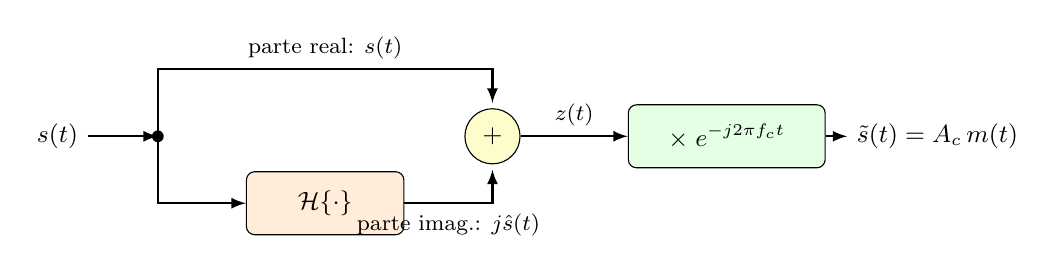
\begin{tikzpicture}[>=latex, scale=0.85,
    bloco/.style={draw, rectangle, rounded corners=3pt, minimum height=0.8cm, font=\small}]

% s(t)
\node[font=\small] (in) at (-4,0) {$s(t)$};

% Branch point
\coordinate (branch) at (-2.5,0);
\fill (branch) circle (2.5pt);

% Upper path: direct (real part)
\draw[->, thick] (in) -- (branch);
\draw[->, thick] (branch) -- ++(0,1) -| node[above, pos=0.25, font=\footnotesize] {parte real: $s(t)$} (2.5, 0.5);

% Lower path: Hilbert (imag part)
\node[bloco, fill=orange!15, minimum width=2cm] (ht) at (0,-1) {$\mathcal{H}\{\cdot\}$};
\draw[->, thick] (branch) |- (ht);
\draw[->, thick] (ht) -| node[below, pos=0.25, font=\footnotesize] {parte imag.: $j\hat{s}(t)$} (2.5,-0.5);

% Combine
\node[draw, circle, fill=yellow!20, minimum size=0.7cm, font=\small] (sum) at (2.5,0) {$+$};

% multiply by exp
\node[bloco, fill=green!10, minimum width=2.5cm] (exp) at (6,0) {$\times\; e^{-j2\pi f_c t}$};
\draw[->, thick] (sum) -- node[above, font=\footnotesize] {$z(t)$} (exp);

% output
\node[font=\small, right] (out) at (7.8,0) {$\tilde{s}(t) = A_c\,m(t)$};
\draw[->, thick] (exp) -- (out);
\end{tikzpicture}
\end{center}

\vspace{0.3cm}

\begin{center}
\colorbox{orange!12}{\parbox{0.85\textwidth}{\centering
Precisa de um \textbf{filtro de Hilbert} (convolução com $\frac{1}{\pi t}$) e de um \textbf{oscilador complexo} ($e^{-j2\pi f_c t}$). Isso é fácil de implementar?
}}
\end{center}
}

\end{frame}

% ============================================
% SLIDE: Dificuldades da abordagem via Hilbert
% ============================================
\begin{frame}{Por que Não Usar Hilbert Diretamente?}

\begin{columns}[T]
\begin{column}{0.48\textwidth}

\textbf{1. Filtro ideal irrealizável}

\vspace{0.1cm}
$H(f) = -j\,\sgn(f)$: descontinuidade em $f=0$

\begin{center}
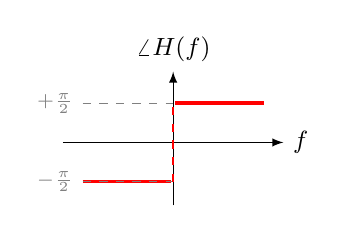
\begin{tikzpicture}[>=latex, scale=0.5]
\draw[->] (-2.8,0) -- (2.8,0) node[right, font=\small] {$f$};
\draw[->] (0,-1.6) -- (0,1.8) node[above, font=\small] {$\angle H(f)$};
\draw[very thick, red] (-2.3,-1.0) -- (-0.05,-1.0);
\draw[very thick, red] (0.05,1.0) -- (2.3,1.0);
\draw[dashed, gray] (-2.3,1.0) -- (0,1.0) node[left, font=\scriptsize, pos=0] {$+\frac{\pi}{2}$};
\draw[dashed, gray] (-2.3,-1.0) -- (0,-1.0) node[left, font=\scriptsize, pos=0] {$-\frac{\pi}{2}$};
\draw[thick, red, dashed] (0,-1.0) -- (0,1.0);
\end{tikzpicture}
\end{center}

\vspace{-0.1cm}
\textbf{2. Oscilador complexo}

$e^{-j2\pi f_c t}$ precisa gerar $\cos$ \textbf{e} $\sin$ e operar sobre sinais complexos.

\end{column}
\begin{column}{0.50\textwidth}

\onslide<2->{
\textbf{3. Na prática:}
\begin{itemize}\setlength{\itemsep}{3pt}
\item Filtros de Hilbert analógicos são difíceis de construir
\item Usado em \textbf{receptores digitais} (DSP)
\item Para receptores \textbf{analógicos}: precisa de solução mais simples
\end{itemize}

\vspace{0.3cm}

\colorbox{green!15}{\parbox{0.95\columnwidth}{\centering
\textbf{Solução prática:} Multiplicar por $\cos(2\pi f_c t)$ e filtrar --- a \textbf{demodulação coerente} faz o mesmo trabalho sem Hilbert!
}}
}

\end{column}
\end{columns}

\end{frame}

% ============================================
% SLIDE: Demodulação Coerente — diagrama + math com overlays
% ============================================
\begin{frame}{Demodulação Coerente do DSB-SC}

\begin{center}
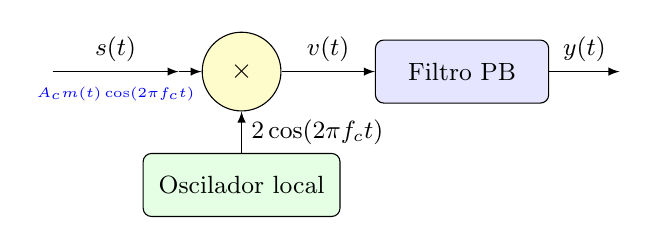
\begin{tikzpicture}[>=latex, scale=0.8,
    bloco/.style={draw, rectangle, rounded corners=3pt, minimum height=0.8cm, font=\small}]
% Sinal recebido
\draw[->] (-3.5,0) -- node[above, font=\small] {$s(t)$} (-1.5,0);
\node[font=\tiny, blue] at (-2.5,-0.35) {$A_c m(t)\cos(2\pi f_c t)$};
% Multiplicador
\node[draw, circle, fill=yellow!20, minimum size=1cm] (mult) at (-0.5,0) {$\times$};
\draw[->] (-1.5,0) -- (mult.west);
% Oscilador local
\node[bloco, fill=green!10, minimum width=2.5cm] (osc) at (-0.5,-1.8) {Oscilador local};
\draw[->] (osc.north) -- node[right, font=\small] {$2\cos(2\pi f_c t)$} (mult.south);
% Filtro passa-baixas
\node[bloco, fill=blue!10, minimum width=2.2cm] (lpf) at (3,0) {Filtro PB};
\draw[->] (mult.east) -- node[above, font=\small] {$v(t)$} (lpf.west);
% Saída
\draw[->] (lpf.east) -- node[above, font=\small] {$y(t)$} (5.5,0);
\end{tikzpicture}
\end{center}

\onslide<2->{
\textbf{Passo 1 --- Multiplicação:}
\[
v(t) = 2A_c m(t) \cos^2(2\pi f_c t) = A_c m(t)\bigl[\underbrace{1}_{\text{banda base}} + \underbrace{\cos(4\pi f_c t)}_{\text{em } 2f_c}\bigr]
\]
}

\onslide<3->{
\textbf{Passo 2 --- Filtro passa-baixas} (remove componente em $2f_c$):
\[
\boxed{y(t) = A_c\, m(t)} \qquad \text{Recuperação perfeita!}
\]
}

\end{frame}

% ============================================
% SLIDE: Demodulação — visão espectral com overlays
% ============================================
\begin{frame}{Demodulação Coerente: Visão Espectral}

\begin{center}
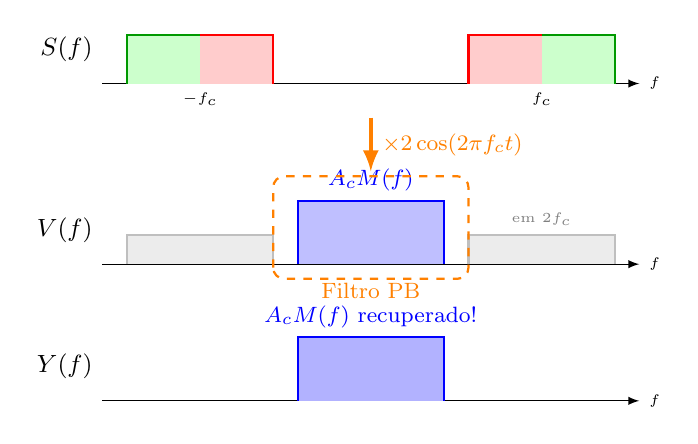
\begin{tikzpicture}[>=latex, scale=0.62]

% S(f) recebido
\begin{scope}[yshift=2.5cm]
\node[left, font=\small] at (-5.5,0.7) {$S(f)$};
\draw[->] (-5.5,0) -- (5.5,0) node[right, font=\tiny] {$f$};
\fill[red!20] (2,0) -- (2,1) -- (3.5,1) -- (3.5,0) -- cycle;
\fill[green!20] (3.5,0) -- (3.5,1) -- (5,1) -- (5,0) -- cycle;
\draw[thick, red] (2,0) -- (2,1) -- (3.5,1);
\draw[thick, green!60!black] (3.5,1) -- (5,1) -- (5,0);
\fill[green!20] (-5,0) -- (-5,1) -- (-3.5,1) -- (-3.5,0) -- cycle;
\fill[red!20] (-3.5,0) -- (-3.5,1) -- (-2,1) -- (-2,0) -- cycle;
\draw[thick, green!60!black] (-5,0) -- (-5,1) -- (-3.5,1);
\draw[thick, red] (-3.5,1) -- (-2,1) -- (-2,0);
\node[below, font=\tiny] at (3.5,0) {$f_c$};
\node[below, font=\tiny] at (-3.5,0) {$-f_c$};
\end{scope}

% Seta
\onslide<2->{
\draw[->, ultra thick, orange] (0,1.8) -- (0,0.7)
  node[midway, right, font=\footnotesize] {$\times 2\cos(2\pi f_c t)$};
}

% V(f) após multiplicação
\onslide<2->{
\begin{scope}[yshift=-1.2cm]
\node[left, font=\small] at (-5.5,0.7) {$V(f)$};
\draw[->] (-5.5,0) -- (5.5,0) node[right, font=\tiny] {$f$};
% Banda base (soma)
\fill[blue!25] (-1.5,0) -- (-1.5,1.3) -- (1.5,1.3) -- (1.5,0) -- cycle;
\draw[thick, blue] (-1.5,0) -- (-1.5,1.3) -- (1.5,1.3) -- (1.5,0);
\node[above, font=\footnotesize, blue] at (0,1.3) {$A_c M(f)$};
% Componentes em 2fc
\fill[gray!15] (3.5,0) -- (3.5,0.6) -- (5,0.6) -- (5,0) -- cycle;
\fill[gray!15] (2,0) -- (2,0.6) -- (3.5,0.6) -- (3.5,0) -- cycle;
\draw[thick, gray!50] (2,0) -- (2,0.6) -- (5,0.6) -- (5,0);
\fill[gray!15] (-5,0) -- (-5,0.6) -- (-2,0.6) -- (-2,0) -- cycle;
\draw[thick, gray!50] (-5,0) -- (-5,0.6) -- (-2,0.6) -- (-2,0);
\node[above, font=\tiny, gray] at (3.5,0.6) {em $2f_c$};
\end{scope}
}

% Filtro PB
\onslide<3->{
\begin{scope}[yshift=-1.2cm]
\draw[thick, dashed, orange, rounded corners] (-2,-0.3) rectangle (2,1.8);
\node[font=\footnotesize, orange] at (0,-0.55) {Filtro PB};
\end{scope}
}

% Y(f) recuperado
\onslide<4->{
\begin{scope}[yshift=-4cm]
\node[left, font=\small] at (-5.5,0.7) {$Y(f)$};
\draw[->] (-5.5,0) -- (5.5,0) node[right, font=\tiny] {$f$};
\fill[blue!30] (-1.5,0) -- (-1.5,1.3) -- (1.5,1.3) -- (1.5,0) -- cycle;
\draw[thick, blue] (-1.5,0) -- (-1.5,1.3) -- (1.5,1.3) -- (1.5,0);
\node[above, font=\footnotesize, blue] at (0,1.3) {$A_c M(f)$ recuperado!};
\end{scope}
}

\end{tikzpicture}
\end{center}

\end{frame}

% %%%%%%%%%%%%%%%%%%%%%%%%%%%%%%%%%%%%%%%%%%%%
% EXERCÍCIOS — AM DSB-SC (Espectro, Potência, DEP)
% %%%%%%%%%%%%%%%%%%%%%%%%%%%%%%%%%%%%%%%%%%%%

\subsection*{Exercícios: Espectro e Potência DSB-SC}

% ============================================
\begin{frame}{Exercício: Espectro e Largura de Banda}

\only<1>{
Um sinal de áudio $m(t)$ com banda $W = 4\,\text{kHz}$ modula uma portadora
$f_c = 1\,\text{MHz}$ usando DSB-SC.

\vspace{0.3cm}

\begin{enumerate}[a)]
\item Qual a faixa de frequências ocupada pelo sinal modulado?
\item Qual a largura de banda $B$?
\item Identifique a LSB e a USB no espectro.
\end{enumerate}
}

\only<2>{
\textbf{Resolução:}

\begin{enumerate}[a)]
\item Faixa: de $f_c - W = 996\,\text{kHz}$ até $f_c + W = 1004\,\text{kHz}$
\item $B = 2W = 2 \times 4 = \boxed{8\,\text{kHz}}$
\item LSB: 996--1000 kHz \quad USB: 1000--1004 kHz
\end{enumerate}

\begin{center}
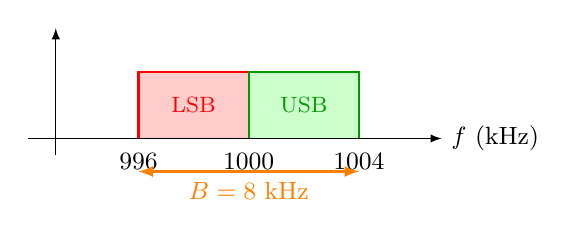
\begin{tikzpicture}[>=latex, scale=0.7]
\draw[->] (-0.5,0) -- (7,0) node[right, font=\small] {$f$ (kHz)};
\draw[->] (0,-0.3) -- (0,2);
\fill[red!20] (1.5,0) -- (1.5,1.2) -- (3.5,1.2) -- (3.5,0) -- cycle;
\fill[green!20] (3.5,0) -- (3.5,1.2) -- (5.5,1.2) -- (5.5,0) -- cycle;
\draw[thick, red] (1.5,0) -- (1.5,1.2) -- (3.5,1.2) -- (3.5,0);
\draw[thick, green!60!black] (3.5,0) -- (3.5,1.2) -- (5.5,1.2) -- (5.5,0);
\node[font=\footnotesize, red] at (2.5,0.6) {LSB};
\node[font=\footnotesize, green!60!black] at (4.5,0.6) {USB};
\node[below, font=\small] at (1.5,-0.1) {996};
\node[below, font=\small] at (3.5,-0.1) {1000};
\node[below, font=\small] at (5.5,-0.1) {1004};
\draw[<->, thick, orange] (1.5,-0.6) -- (5.5,-0.6) node[midway, below, font=\small] {$B=8$ kHz};
\end{tikzpicture}
\end{center}
}

\end{frame}

% ============================================
\begin{frame}{Exercício: Potência com Dois Tons}

\only<1>{
Um transmissor DSB-SC opera com $A_c = 20\,\text{V}$ e mensagem
$m(t) = 3\cos(2\pi \cdot 1000\, t) + 2\cos(2\pi \cdot 3000\, t)$.

\vspace{0.3cm}

\begin{enumerate}[a)]
\item Calcule a potência da mensagem $P_m$.
\item Calcule a potência do sinal transmitido $P_s$.
\item Quantas componentes espectrais existem e em que frequências?
\end{enumerate}
}

\only<2>{
\textbf{a) Potência da mensagem:}
\[
P_m = \frac{3^2}{2} + \frac{2^2}{2} = 4.5 + 2 = \boxed{6.5\,\text{W}}
\]

\textbf{b) Potência transmitida:}
\[
P_s = \frac{A_c^2 P_m}{2} = \frac{400 \times 6.5}{2} = \boxed{1300\,\text{W}}
\]

\textbf{c) Componentes:} 4 componentes espectrais

\begin{center}
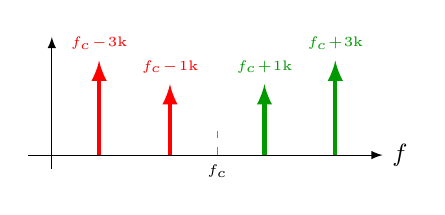
\begin{tikzpicture}[>=latex, scale=0.6]
\draw[->] (-0.5,0) -- (7,0) node[right, font=\small] {$f$};
\draw[->] (0,-0.3) -- (0,2.5);
\draw[thick, red, ->, line width=1.5pt] (1,0) -- (1,2) node[above, font=\tiny] {$f_c\!-\!3$k};
\draw[thick, red, ->, line width=1.5pt] (2.5,0) -- (2.5,1.5) node[above, font=\tiny] {$f_c\!-\!1$k};
\draw[thick, green!60!black, ->, line width=1.5pt] (4.5,0) -- (4.5,1.5) node[above, font=\tiny] {$f_c\!+\!1$k};
\draw[thick, green!60!black, ->, line width=1.5pt] (6,0) -- (6,2) node[above, font=\tiny] {$f_c\!+\!3$k};
\draw[dashed, gray] (3.5,0) -- (3.5,0.5);
\node[below, font=\tiny] at (3.5,0) {$f_c$};
\end{tikzpicture}
\end{center}
}

\end{frame}

% ============================================
\begin{frame}{Exercício: Densidade Espectral de Potência}

\only<1>{
A mensagem $m(t)$ tem densidade espectral de potência (DEP):
\[
S_m(f) = \begin{cases}
\frac{S_0}{2W}\left(1 - \frac{|f|}{W}\right) & |f| \leq W \\
0 & |f| > W
\end{cases}
\]
com $S_0 = 4\,\text{W}$ e $W = 5\,\text{kHz}$. A portadora tem $A_c = 10\,\text{V}$, $f_c = 100\,\text{kHz}$.

\vspace{0.2cm}

\begin{enumerate}[a)]
\item Esboce $S_m(f)$ e calcule a potência $P_m$ da mensagem.
\item Determine $S_s(f)$ do sinal DSB-SC modulado.
\item Calcule $P_s$ diretamente pela DEP e verifique com $P_s = \frac{A_c^2 P_m}{2}$.
\end{enumerate}
}

\only<2>{
\textbf{a)} $P_m = \int_{-W}^{W} S_m(f)\, df = S_0 \times \frac{1}{2} \times 1 = \frac{S_0}{2} = \boxed{2\,\text{W}}$

\begin{center}
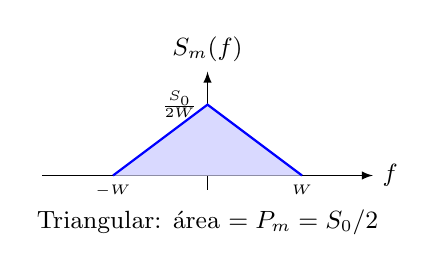
\begin{tikzpicture}[>=latex, scale=0.6]
% Sm(f)
\draw[->] (-3.5,0) -- (3.5,0) node[right, font=\small] {$f$};
\draw[->] (0,-0.3) -- (0,2.2) node[above, font=\small] {$S_m(f)$};
\fill[blue!15] (-2,0) -- (0,1.5) -- (2,0) -- cycle;
\draw[thick, blue] (-2,0) -- (0,1.5) -- (2,0);
\node[below, font=\tiny] at (-2,0) {$-W$};
\node[below, font=\tiny] at (2,0) {$W$};
\node[left, font=\tiny] at (0,1.5) {$\frac{S_0}{2W}$};
\node[font=\small] at (0,-1) {Triangular: área $= P_m = S_0/2$};
\end{tikzpicture}
\end{center}
}

\only<3>{
\textbf{b)} DEP do sinal modulado $s(t) = A_c m(t)\cos(2\pi f_c t)$:
\[
\boxed{S_s(f) = \frac{A_c^2}{4}[S_m(f - f_c) + S_m(f + f_c)]}
\]

\begin{center}
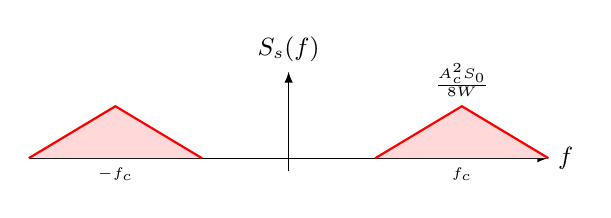
\begin{tikzpicture}[>=latex, scale=0.55]
\draw[->] (-6,0) -- (6,0) node[right, font=\small] {$f$};
\draw[->] (0,-0.3) -- (0,2) node[above, font=\small] {$S_s(f)$};
% Em +fc
\fill[red!15] (2,0) -- (4,1.2) -- (6,0) -- cycle;
\draw[thick, red] (2,0) -- (4,1.2) -- (6,0);
\node[below, font=\tiny] at (4,0) {$f_c$};
% Em -fc
\fill[red!15] (-6,0) -- (-4,1.2) -- (-2,0) -- cycle;
\draw[thick, red] (-6,0) -- (-4,1.2) -- (-2,0);
\node[below, font=\tiny] at (-4,0) {$-f_c$};
\node[above, font=\tiny] at (4,1.2) {$\frac{A_c^2 S_0}{8W}$};
\end{tikzpicture}
\end{center}

\textbf{c)} $P_s = \int S_s(f)\,df = \frac{A_c^2}{2} P_m = \frac{100}{2}\times 2 = \boxed{100\,\text{W}}$ \checkmark
}

\end{frame}

% ============================================
% SLIDE: Erro de Fase — matemática com overlays
% ============================================
\begin{frame}{Efeito de Erro de Fase na Demodulação}

\only<1>{
\textbf{Oscilador local com erro de fase:} $2\cos(2\pi f_c t + \theta)$

\vspace{0.2cm}

Após multiplicação:
\[
v(t) = 2A_c m(t)\cos(2\pi f_c t)\cos(2\pi f_c t + \theta)
\]

Usando $\cos A \cos B = \frac{1}{2}[\cos(A\!-\!B) + \cos(A\!+\!B)]$:
\[
v(t) = A_c m(t)\bigl[\underbrace{\cos\theta}_{\text{banda base}} + \underbrace{\cos(4\pi f_c t + \theta)}_{\text{removido pelo LPF}}\bigr]
\]

Após filtro passa-baixas:
\[
\boxed{y(t) = A_c\, m(t) \cos\theta}
\]
}

\only<2>{
\[
\boxed{y(t) = A_c\, m(t) \cos\theta}
\]

\vspace{0.3cm}

\begin{center}
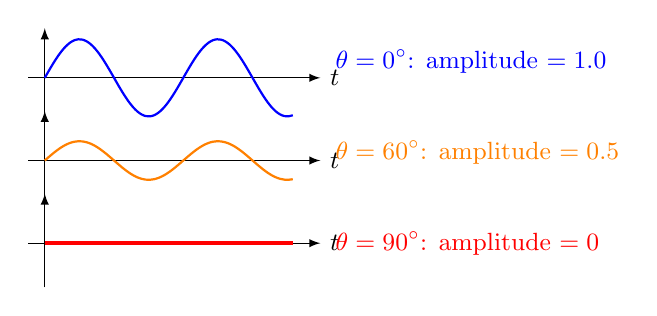
\begin{tikzpicture}[>=latex, scale=0.7]
% theta = 0
\begin{scope}[yshift=1.5cm]
\draw[->] (-0.3,0) -- (5,0) node[right, font=\small] {$t$};
\draw[->] (0,-0.8) -- (0,0.9);
\draw[thick, blue, smooth] plot[domain=0:4.5, samples=60]
  (\x, {0.7*sin(2.5*\x r)});
\node[right, font=\small, blue] at (5.1,0.3) {$\theta = 0^{\circ}$: amplitude $= 1.0$};
\end{scope}
% theta = 60
\begin{scope}[yshift=0cm]
\draw[->] (-0.3,0) -- (5,0) node[right, font=\small] {$t$};
\draw[->] (0,-0.8) -- (0,0.9);
\draw[thick, orange, smooth] plot[domain=0:4.5, samples=60]
  (\x, {0.35*sin(2.5*\x r)});
\node[right, font=\small, orange] at (5.1,0.15) {$\theta = 60^{\circ}$: amplitude $= 0.5$};
\end{scope}
% theta = 90
\begin{scope}[yshift=-1.5cm]
\draw[->] (-0.3,0) -- (5,0) node[right, font=\small] {$t$};
\draw[->] (0,-0.8) -- (0,0.9);
\draw[thick, red, line width=1.5pt] (0,0) -- (4.5,0);
\node[right, font=\small, red] at (5.1,0) {$\theta = 90^{\circ}$: amplitude $= 0$};
\end{scope}
\end{tikzpicture}
\end{center}
}

\end{frame}

% ============================================
% SLIDE: Erro de fase — curva cos(θ) e valores
% ============================================
\begin{frame}{Atenuação por Erro de Fase: $\cos\theta$}

\begin{columns}[T]
\begin{column}{0.50\textwidth}

\begin{center}
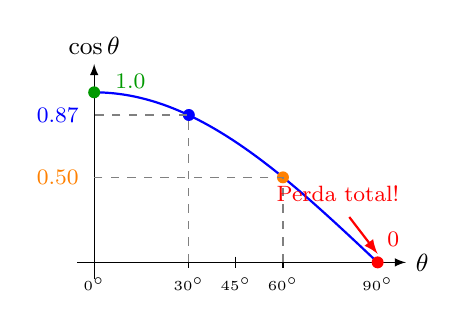
\begin{tikzpicture}[>=latex, scale=0.72]
\draw[->] (-0.3,0) -- (5.5,0) node[right, font=\small] {$\theta$};
\draw[->] (0,-0.3) -- (0,3.5) node[above, font=\small] {$\cos\theta$};

% Curva cos(theta) de 0 a 90
\draw[thick, blue, smooth] plot[domain=0:5, samples=100]
  (\x, {3*cos(\x/5*90)});

% Marcas no eixo x
\foreach \ang/\pos in {0/0, 30/1.67, 45/2.5, 60/3.33, 90/5} {
  \draw (\pos,0.1) -- (\pos,-0.1) node[below, font=\tiny] {$\ang^{\circ}$};
}

% Pontos e valores
\onslide<2->{
\fill[green!60!black] (0,3) circle (3pt);
\node[right, font=\footnotesize, green!60!black] at (0.2,3.2) {$1.0$};
}

\onslide<3->{
\fill[blue] (1.67,2.6) circle (3pt);
\draw[dashed, gray] (1.67,0) -- (1.67,2.6) -- (0,2.6);
\node[left, font=\footnotesize, blue] at (-0.1,2.6) {$0.87$};
}

\onslide<4->{
\fill[orange] (3.33,1.5) circle (3pt);
\draw[dashed, gray] (3.33,0) -- (3.33,1.5) -- (0,1.5);
\node[left, font=\footnotesize, orange] at (-0.1,1.5) {$0.50$};
}

\onslide<5->{
\fill[red] (5,0) circle (3pt);
\node[above right, font=\footnotesize, red] at (5,0.1) {$0$};
\draw[thick, red, ->] (4.5,0.8) -- (5,0.15);
\node[above, font=\footnotesize, red] at (4.3,0.9) {Perda total!};
}

\end{tikzpicture}
\end{center}

\end{column}
\begin{column}{0.48\textwidth}

\onslide<2->{
\begin{center}
\footnotesize
\begin{tabular}{c c c}
\textbf{Erro $\theta$} & $\cos\theta$ & \textbf{Atenuação} \\
\hline
$0^{\circ}$  & 1.00 & 0 dB \\
$10^{\circ}$ & 0.98 & $-$0.1 dB \\
$30^{\circ}$ & 0.87 & $-$1.2 dB \\
$45^{\circ}$ & 0.71 & $-$3.0 dB \\
$60^{\circ}$ & 0.50 & $-$6.0 dB \\
$90^{\circ}$ & 0    & $-\infty$ dB \\
\end{tabular}
\end{center}
}

\onslide<5->{
\vspace{0.3cm}
\textbf{Conclusão:}

Sincronização de fase é \textbf{crítica} para DSB-SC. Erros acima de $30^{\circ}$ já causam degradação significativa.
}

\end{column}
\end{columns}

\end{frame}

% ============================================
% SLIDE: Causas práticas do erro de sincronismo
% ============================================
\begin{frame}{Erro de Sincronismo: Causas Práticas}

\only<1>{
\textbf{1. Instabilidade do oscilador local}

\begin{itemize}
\item Envelhecimento do cristal de referência
\item Variação de temperatura ambiente
\item Ruído de fase intrínseco do oscilador
\end{itemize}

\vspace{0.5cm}

\begin{center}
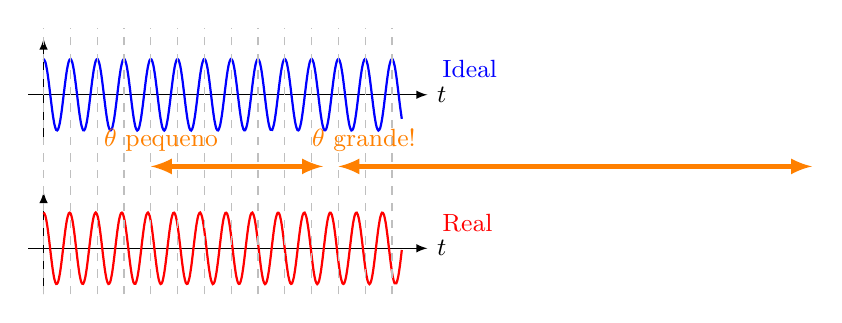
\begin{tikzpicture}[>=latex, scale=0.65]
% Frequência mais baixa (12 rad/s) para ver os ciclos claramente
% Portadora ideal
\begin{scope}[yshift=1.5cm]
\draw[->] (-0.3,0) -- (7.5,0) node[right, font=\small] {$t$};
\draw[->] (0,-0.9) -- (0,1.1);
\draw[thick, blue, smooth] plot[domain=0:7, samples=200]
  (\x, {0.7*cos(12*\x r)});
\node[right, font=\small, blue] at (7.6,0.5) {Ideal};
\end{scope}
% Portadora com drift GRANDE: fase cresce 3*pi ao longo do tempo
% Começa alinhado, termina quase em anti-fase
\begin{scope}[yshift=-1.5cm]
\draw[->] (-0.3,0) -- (7.5,0) node[right, font=\small] {$t$};
\draw[->] (0,-0.9) -- (0,1.1);
\draw[thick, red, smooth] plot[domain=0:7, samples=200]
  (\x, {0.7*cos(12*\x r + 135*\x/7)});
\node[right, font=\small, red] at (7.6,0.5) {Real};
\end{scope}
% Linhas verticais de referência nos picos do ideal
% cos(12x) = 1 quando 12x = 360n => x = 360n/12 = 30n graus
% Em radianos do TikZ: picos em x = 2*pi*n/12*180/pi... simplificando:
% Picos do cos(12x deg) ocorrem a cada 360/12 = 30 unidades TikZ...
% Mas TikZ usa graus: cos(12*x r) => 12*x em radianos
% Pico quando 12*x = 2*pi*n => x = pi*n/6 ≈ 0.524*n
\foreach \n in {0,1,...,13} {
  \draw[gray!50, dashed] ({3.14159*\n/6},-2.4) -- ({3.14159*\n/6},2.8);
}
% Setas mostrando desvio crescente entre picos
% No meio (x~3.5): desvio já é perceptível
\draw[<->, ultra thick, orange] ({3.14159*4/6},0.1) -- ({3.14159*4/6 + 135*3.14159*4/6 / (7*12)},0.1);
\node[above, font=\small, orange] at ({3.14159*4/6 + 0.2},0.2) {$\theta$ pequeno};
% No final (x~6): desvio é grande
\draw[<->, ultra thick, orange] ({3.14159*11/6},0.1) -- ({3.14159*11/6 + 135*3.14159*11/6 / (7*12)},0.1);
\node[above, font=\small, orange] at ({3.14159*11/6 + 0.5},0.2) {$\theta$ grande!};
\end{tikzpicture}
\end{center}
}

\only<2>{
\textbf{2. Efeito Doppler}

\begin{itemize}
\item Transmissor ou receptor em movimento
\item Desvio de frequência: $\Delta f = \dfrac{v}{c}\, f_c$
\item Ex.: $v = 100$ km/h, $f_c = 1$ GHz $\Rightarrow$ $\Delta f \approx 93$ Hz
\end{itemize}

\vspace{0.5cm}

\textbf{3. Propagação multipercurso}

\begin{itemize}
\item Reflexões em obstáculos criam cópias com atrasos variáveis
\item Canal variante no tempo $\rightarrow$ fase do sinal recebido flutua
\end{itemize}
}

\only<3>{
\textbf{Recuperação de portadora no receptor}

\vspace{0.3cm}

\begin{center}
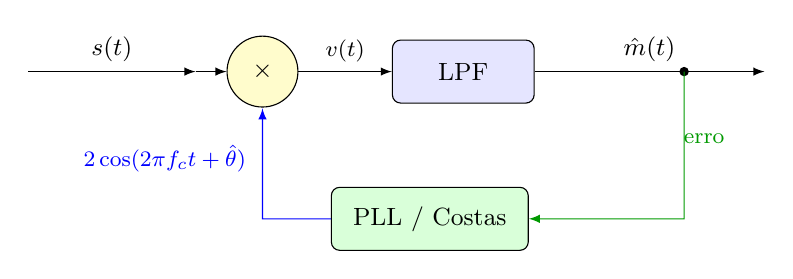
\begin{tikzpicture}[>=latex, scale=0.85,
    bloco/.style={draw, rectangle, rounded corners=3pt, minimum height=0.8cm, font=\small}]
% Sinal recebido
\draw[->] (-3,0) -- node[above, font=\small] {$s(t)$} (-0.5,0);
% Multiplicador
\node[draw, circle, fill=yellow!20, minimum size=0.9cm, font=\small] (mult) at (0.5,0) {$\times$};
\draw[->] (-0.5,0) -- (mult.west);
% LPF
\node[bloco, fill=blue!10, minimum width=1.8cm] (lpf) at (3.5,0) {LPF};
\draw[->] (mult.east) -- node[above, font=\footnotesize] {$v(t)$} (lpf.west);
% Saída
\draw[->] (lpf.east) -- node[above, font=\small] {$\hat{m}(t)$} (8,0);
% Ponto de derivação após LPF (mais à frente)
\coordinate (tap) at (6.8,0);
\fill (tap) circle (2pt);
% PLL abaixo, centrado entre mult e saída
\node[bloco, fill=green!15, minimum width=2.5cm] (pll) at (3,-2.2) {PLL / Costas};
% Realimentação: desce da saída, vai ao PLL
\draw[->, green!60!black] (tap) -- (6.8,-2.2) -- (pll.east);
\node[font=\footnotesize, green!60!black] at (7.1,-1) {erro};
% PLL gera oscilador local: sai pela esquerda, sobe ao multiplicador
\draw[->, blue] (pll.west) -- (0.5,-2.2) -- (0.5,-0.55);
\node[font=\footnotesize, blue, left] at (0.4,-1.3) {$2\cos(2\pi f_c t + \hat{\theta})$};
\end{tikzpicture}
\end{center}

\vspace{0.1cm}

O PLL estima $\hat{\theta} \approx \theta$ e ajusta o oscilador local continuamente

\textbf{Circuitos:} PLL, laço de Costas, squaring loop
}

\end{frame}

% ============================================
% SLIDE: Modelagem da perda de fase
% ============================================
\begin{frame}{Modelagem: Perda de Fase no Receptor}

\only<1>{
\textbf{Sinal recebido:} $r(t) = A_c\, m(t)\cos(2\pi f_c t + \phi(t))$

onde $\phi(t)$ é a fase desconhecida (drift + Doppler + canal)

\vspace{0.3cm}

\textbf{Oscilador local:} $c_L(t) = 2\cos(2\pi f_c t + \hat{\phi}(t))$

onde $\hat{\phi}(t)$ é a estimativa da fase

\vspace{0.3cm}

\textbf{Saída do demodulador} (após LPF):
\[
y(t) = A_c\, m(t)\cos\bigl(\phi(t) - \hat{\phi}(t)\bigr) = A_c\, m(t)\cos(\theta_e(t))
\]

onde $\theta_e(t) = \phi(t) - \hat{\phi}(t)$ é o \textbf{erro de fase}

\vspace{0.2cm}
\footnotesize
Nota: a saída do demodulador depende de $\cos(\theta_e)$. Para \textbf{estimar} $\theta_e$ e corrigi-lo, o PLL usa internamente um detector em \textbf{quadratura} ($-\sin$), que produz $\sin(\theta_e)$ --- uma função ímpar que indica a \textit{direção} do erro.
}

\only<2>{
\textbf{Objetivo:} minimizar $\theta_e(t) = \phi(t) - \hat{\phi}(t)$

\vspace{0.3cm}

\begin{center}
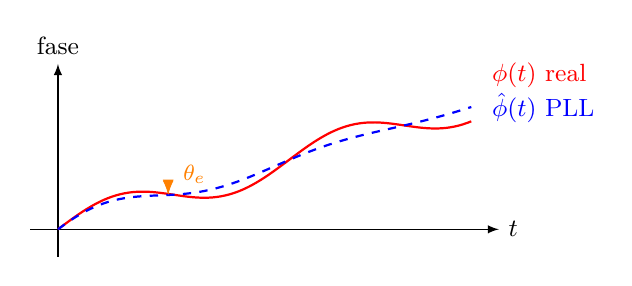
\begin{tikzpicture}[>=latex, scale=0.7]
\draw[->] (-0.5,0) -- (8,0) node[right, font=\small] {$t$};
\draw[->] (0,-0.5) -- (0,3) node[above, font=\small] {fase};
% phi(t) — fase real (drift linear)
\draw[thick, red, smooth] plot[domain=0:7.5, samples=100]
  (\x, {0.3*\x + 0.3*sin(1.5*\x r)});
\node[right, font=\small, red] at (7.7,2.8) {$\phi(t)$ real};
% phi_hat(t) — estimativa do PLL (segue com atraso)
\draw[thick, blue, smooth, dashed] plot[domain=0:7.5, samples=100]
  (\x, {0.3*\x + 0.3*sin(1.5*\x r) * exp(-0.3*\x) });
\node[right, font=\small, blue] at (7.7,2.2) {$\hat{\phi}(t)$ PLL};
% Erro
\draw[<->, thick, orange] (2, {0.3*2 + 0.3*sin(3 r)}) -- (2, {0.3*2 + 0.3*sin(3 r)*exp(-0.6)});
\node[right, font=\footnotesize, orange] at (2.1,1) {$\theta_e$};
\end{tikzpicture}
\end{center}

\textbf{Sem PLL:} $\hat{\phi}(t) = 0$, $\theta_e$ cresce $\rightarrow$ sinal perdido

\textbf{Com PLL:} $\hat{\phi}(t) \rightarrow \phi(t)$, $\theta_e \rightarrow 0$ $\rightarrow$ sinal recuperado
}

\end{frame}

% ============================================
% SLIDE: Arquitetura do PLL — overlay progressivo
% ============================================
\begin{frame}{Arquitetura do PLL (Phase-Locked Loop)}

\begin{center}
\begin{tikzpicture}[>=latex, scale=0.65,
    bloco/.style={draw, rectangle, rounded corners=2pt, minimum height=0.7cm,
                  minimum width=1.6cm, font=\footnotesize, thick},
    destaque/.style={draw, rectangle, rounded corners=2pt, minimum height=0.7cm,
                  minimum width=1.6cm, font=\footnotesize, very thick}]
% Detector de fase
\only<1>{\node[destaque, fill=yellow!40, draw=red, line width=1.5pt] (pd) at (0,0) {\begin{tabular}{c}\tiny Detector\\\tiny de Fase\end{tabular}};}
\only<2->{\node[bloco, fill=yellow!15] (pd) at (0,0) {\begin{tabular}{c}\tiny Detector\\\tiny de Fase\end{tabular}};}
% Filtro de loop
\only<2>{\node[destaque, fill=blue!30, draw=red, line width=1.5pt] (lf) at (3.5,0) {\begin{tabular}{c}\tiny Filtro\\\tiny $F(s)$\end{tabular}};}
\only<1>{\node[bloco, fill=blue!8] (lf) at (3.5,0) {\begin{tabular}{c}\tiny Filtro\\\tiny $F(s)$\end{tabular}};}
\only<3->{\node[bloco, fill=blue!15] (lf) at (3.5,0) {\begin{tabular}{c}\tiny Filtro\\\tiny $F(s)$\end{tabular}};}
% VCO
\only<3>{\node[destaque, fill=green!30, draw=red, line width=1.5pt] (vco) at (3.5,-1.6) {\tiny VCO};}
\only<1-2>{\node[bloco, fill=green!8] (vco) at (3.5,-1.6) {\tiny VCO};}
\only<4->{\node[bloco, fill=green!15] (vco) at (3.5,-1.6) {\tiny VCO};}
% Entrada
\draw[->] (-2.2,0.15) -- node[above, font=\tiny] {$r(t)$} (pd.west |- 0,0.15);
% Conexões
\draw[->] (pd.east) -- node[above, font=\tiny] {$e(t)$} (lf.west);
\coordinate (corner) at (6.5,0);
\draw (lf.east) -- (corner);
\draw[->] (corner) -- (6.5,-1.6) -- (vco.east);
\draw[->] (vco.west) -- (0,-1.6) -- (pd.south);
\node[font=\tiny, blue] at (1.3,-1.85) {$c_L(t) = -2\sin(2\pi f_c t + \hat{\phi})$};
\fill (corner) circle (2pt);
\draw[->] (corner) -- ++(2,0) node[right, font=\tiny] {$v_c(t)$};
\end{tikzpicture}
\end{center}

\vspace{-0.3cm}

% --- Overlay 1: Detector de Fase ---
\only<1>{
\textbf{Detector de Fase (PD):} multiplica $r(t)$ pela saída do VCO e filtra

\vspace{-0.1cm}
\[
r(t) \times c_L(t) = \underbrace{A_c m(t)\cos(2\pi f_c t + \phi)}_{\text{sinal recebido}} \times \underbrace{\bigl(-2\sin(2\pi f_c t + \hat{\phi})\bigr)}_{\text{VCO (em quadratura)}}
\]

\vspace{-0.3cm}
Após o LPF (remove termo em $2f_c$):
\vspace{-0.2cm}
\[
e(t) = K_d\sin\!\bigl(\underbrace{\phi - \hat{\phi}}_{\theta_e}\bigr)
\]

\vspace{-0.3cm}
Para erros pequenos ($\theta_e \ll 1$): \quad
$\boxed{e(t) \approx K_d\, \theta_e(t)}$, \quad $\theta_e = \phi - \hat{\phi}$
}

% --- Overlay 2: Filtro de Loop ---
\only<2>{
\textbf{Filtro de Loop $F(s)$:} suaviza o erro e define a dinâmica
\[
\boxed{V_c(s) = F(s) \cdot E(s)}
\]
\begin{itemize}
\item $F(s) = 1$: PLL de 1ª ordem (simples, erro em regime para rampa)
\item $F(s) = \frac{1 + \tau_2 s}{\tau_1 s}$: 2ª ordem (erro zero para rampa)
\end{itemize}
}

% --- Overlay 3: VCO ---
\only<3>{
\textbf{VCO:} frequência instantânea varia com $v_c(t)$
\[
\boxed{\frac{d\hat{\phi}}{dt} = 2\pi K_v\, v_c(t)}
\]
\begin{itemize}
\item $K_v$: sensibilidade do VCO (Hz/V)
\item $v_c > 0$: frequência sobe \quad $v_c < 0$: frequência desce
\end{itemize}
}

% --- Overlay 4: Resumo completo ---
\only<4>{
\textbf{Ciclo completo do PLL:}

\vspace{0.2cm}

\begin{center}
$\theta_e = \phi - \hat{\phi}$
\enspace$\xrightarrow{\text{PD}}$\enspace
$e \approx K_d\,\theta_e$
\enspace$\xrightarrow{F(s)}$\enspace
$v_c$
\enspace$\xrightarrow{\text{VCO}}$\enspace
$\dfrac{d\hat{\phi}}{dt} = 2\pi K_v v_c$
\enspace$\rightarrow$\enspace
$\hat{\phi} \rightarrow \phi$
\end{center}

\vspace{0.3cm}

A \textbf{realimentação negativa} faz $\theta_e \rightarrow 0$: o VCO ``persegue'' a fase da entrada até travar
}

\end{frame}

% ============================================
% SLIDE: Aproximação linear do PLL
% ============================================
\begin{frame}{Aproximação Linear: Quando Vale $\sin(\theta_e) \approx \theta_e$?}

\only<1>{
\begin{center}
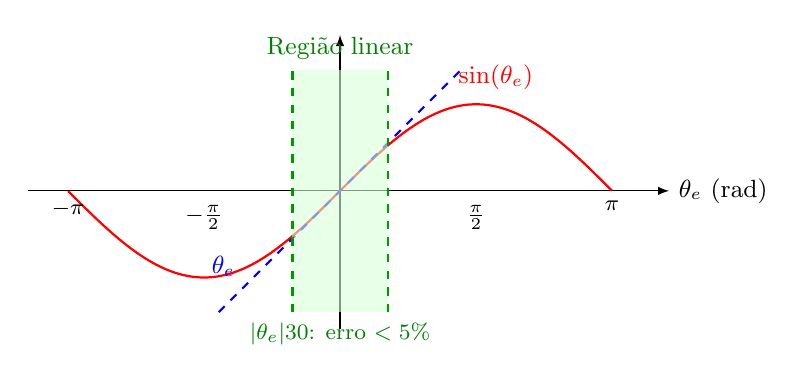
\begin{tikzpicture}[>=latex, scale=1.1]
\draw[->] (-3.6,0) -- (3.8,0) node[right, font=\small] {$\theta_e$ (rad)};
\draw[->] (0,-1.6) -- (0,1.8);
% sin(theta)
\draw[thick, red, smooth, domain=-3.14:3.14, samples=120] plot (\x, {sin(\x r)});
\node[red, font=\small, above] at (1.8,1.05) {$\sin(\theta_e)$};
% theta (linear)
\draw[thick, blue, dashed, domain=-1.4:1.4] plot (\x, {\x});
\node[blue, font=\small, above left] at (-1.1,-1.1) {$\theta_e$};
% Shaded valid region
\fill[green!15, opacity=0.6] (-0.55,-1.4) rectangle (0.55,1.4);
\draw[green!60!black, thick, dashed] (-0.55,-1.4) -- (-0.55,1.4);
\draw[green!60!black, thick, dashed] (0.55,-1.4) -- (0.55,1.4);
% Labels
\node[below, font=\footnotesize] at (3.14,0) {$\pi$};
\node[below, font=\footnotesize] at (-3.14,0) {$-\pi$};
\node[below, font=\footnotesize] at (1.57,-0.05) {$\frac{\pi}{2}$};
\node[below, font=\footnotesize] at (-1.57,-0.05) {$-\frac{\pi}{2}$};
% Green region label
\node[green!50!black, font=\small, align=center] at (0,1.65) {Região linear};
\node[green!50!black, font=\footnotesize] at (0,-1.65) {$|\theta_e| \lesssim 30°$: erro $< 5\%$};
\end{tikzpicture}
\end{center}

Na região sombreada, $\sin(\theta_e) \approx \theta_e$ e o PLL pode ser analisado como sistema \textbf{linear}.
}

\only<2>{
\begin{columns}[c]
\begin{column}{0.45\textwidth}
\begin{center}
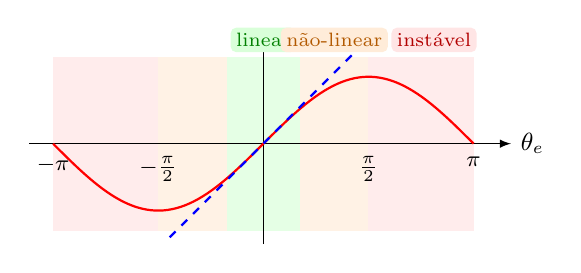
\begin{tikzpicture}[>=latex, scale=0.85]
% Regions with colors (draw first, behind curves)
\fill[green!20, opacity=0.5] (-0.55,-1.3) rectangle (0.55,1.3);
\fill[orange!20, opacity=0.5] (0.55,-1.3) rectangle (1.57,1.3);
\fill[orange!20, opacity=0.5] (-1.57,-1.3) rectangle (-0.55,1.3);
\fill[red!15, opacity=0.5] (1.57,-1.3) rectangle (3.14,1.3);
\fill[red!15, opacity=0.5] (-3.14,-1.3) rectangle (-1.57,1.3);
% Axes
\draw[->] (-3.5,0) -- (3.7,0) node[right, font=\small] {$\theta_e$};
\draw[->] (0,-1.5) -- (0,1.7);
% sin(theta)
\draw[thick, red, smooth, domain=-3.14:3.14, samples=100] plot (\x, {sin(\x r)});
% theta (linear)
\draw[thick, blue, dashed, domain=-1.4:1.4] plot (\x, {\x});
% Region labels — above the plot, spread out
\node[green!50!black, font=\scriptsize, fill=green!15, rounded corners=2pt, inner sep=2pt] at (0,1.55) {linear};
\node[orange!70!black, font=\scriptsize, fill=orange!15, rounded corners=2pt, inner sep=2pt] at (1.06,1.55) {não-linear};
\node[red!70!black, font=\scriptsize, fill=red!10, rounded corners=2pt, inner sep=2pt] at (2.55,1.55) {instável};
% Tick labels
\node[below, font=\footnotesize] at (3.14,-0.05) {$\pi$};
\node[below, font=\footnotesize] at (-3.14,-0.05) {$-\pi$};
\node[below, font=\footnotesize] at (1.57,-0.05) {$\frac{\pi}{2}$};
\node[below, font=\footnotesize] at (-1.57,-0.05) {$-\frac{\pi}{2}$};
\end{tikzpicture}
\end{center}
\end{column}
\begin{column}{0.53\textwidth}

\textbf{\color{green!50!black} Região linear} ($|\theta_e| < 30°$):
\begin{itemize}\setlength{\itemsep}{1pt}
\item $\sin(\theta_e) \approx \theta_e$ (erro $< 5\%$)
\item Análise por Laplace válida
\end{itemize}

\vspace{0.2cm}

\textbf{\color{orange!70!black} Região não-linear} ($30° < |\theta_e| < 90°$):
\begin{itemize}\setlength{\itemsep}{1pt}
\item $\sin$ satura $\to$ ganho efetivo cai
\item PLL ainda converge, mas mais lento
\end{itemize}

\vspace{0.2cm}

\textbf{\color{red!70!black} Região instável} ($|\theta_e| > 90°$):
\begin{itemize}\setlength{\itemsep}{1pt}
\item Sinal de erro \textbf{inverte}
\item PLL perde travamento
\item Precisa \textbf{recapturar} a fase
\end{itemize}

\end{column}
\end{columns}
}


\end{frame}

% ============================================
% SLIDE: Equação do PLL — derivação
% ============================================
\begin{frame}{Equação do PLL: Derivação}

\only<1>{
\textbf{Erro de fase:} $\theta_e(t) = \phi(t) - \hat{\phi}(t)$

\vspace{0.2cm}

\textbf{Detector de fase} (erros pequenos):
\[
e(t) \approx K_d\, \theta_e(t) = K_d[\phi(t) - \hat{\phi}(t)]
\]

\textbf{Filtro de loop:}
\[
v_c(t) = f(t) \ast e(t)
\]

\textbf{VCO:}
\[
\frac{d\hat{\phi}}{dt} = 2\pi K_v\, v_c(t)
\]

Combinando: $\dfrac{d\hat{\phi}}{dt} = 2\pi K_v \bigl[f(t) \ast K_d\,\theta_e(t)\bigr]$
}

\only<2>{
\textbf{Passando ao domínio de Laplace} (propriedades: convolução $\to$ produto, derivada $\to$ $s$):

\vspace{0.1cm}

\begin{tabular}{l @{\;$\xrightarrow{\;\mathcal{L}\;}$\;} l l}
$e(t) = K_d\,\theta_e(t)$ & $E(s) = K_d\,\Theta_e(s)$ & \footnotesize (linearidade) \\[4pt]
$v_c(t) = f(t) \ast e(t)$ & $V_c(s) = F(s)\cdot E(s)$ & \footnotesize (convolução $\to$ produto) \\[4pt]
$\dfrac{d\hat{\phi}}{dt} = 2\pi K_v\, v_c(t)$ & $s\,\hat{\Phi}(s) = 2\pi K_v\, V_c(s)$ & \footnotesize (derivada $\to$ $s$)
\end{tabular}

\vspace{0.15cm}

Encadeando (e absorvendo $2\pi$ em $K_v$ por convenção):
\vspace{-0.15cm}
\[
\hat{\Phi}(s) = \frac{K_v}{s} \cdot F(s) \cdot K_d \cdot \Theta_e(s)
\]

\vspace{-0.3cm}

Como $\Theta_e(s) = \Phi(s) - \hat{\Phi}(s)$:
\vspace{-0.15cm}
\[
\hat{\Phi}(s) = \frac{K_d K_v F(s)}{s}\bigl[\Phi(s) - \hat{\Phi}(s)\bigr]
\]
}

\only<3>{
\textbf{Isolando $\hat{\Phi}(s)$:}
\vspace{-0.2cm}
\[
\hat{\Phi}(s)\left[1 + \frac{K_d K_v F(s)}{s}\right] = \frac{K_d K_v F(s)}{s}\,\Phi(s)
\qquad\Rightarrow\qquad
\hat{\Phi}(s)\cdot\frac{s + K_d K_v F(s)}{s} = \frac{K_d K_v F(s)}{s}\,\Phi(s)
\]

\vspace{-0.1cm}

\textbf{Função de transferência em malha fechada:}
\vspace{-0.1cm}
\[
\boxed{H(s) = \frac{\hat{\Phi}(s)}{\Phi(s)} = \frac{K_d K_v F(s)}{s + K_d K_v F(s)}}
\]

\vspace{-0.1cm}

\begin{center}
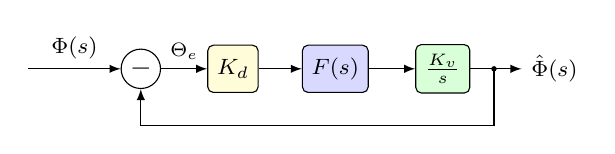
\begin{tikzpicture}[>=latex, scale=0.65,
    bloco/.style={draw, rectangle, rounded corners=2pt, minimum height=0.6cm, font=\footnotesize}]
\node[draw, circle, minimum size=0.5cm, inner sep=0pt] (sum) at (0,0) {$-$};
\draw[->] (-2.2,0) -- node[above, font=\footnotesize] {$\Phi(s)$} (sum.west);
\node[bloco, fill=yellow!15] (kd) at (1.8,0) {$K_d$};
\draw[->] (sum.east) -- node[above, font=\scriptsize] {$\Theta_e$} (kd.west);
\node[bloco, fill=blue!15] (fs) at (3.8,0) {$F(s)$};
\draw[->] (kd.east) -- (fs.west);
\node[bloco, fill=green!15] (kv) at (5.9,0) {$\frac{K_v}{s}$};
\draw[->] (fs.east) -- (kv.west);
\draw[->] (kv.east) -- ++(1.0,0) node[right, font=\footnotesize] {$\hat{\Phi}(s)$};
\coordinate (tap) at (6.9,0);
\fill (tap) circle (1.5pt);
\draw[->] (tap) |- (0,-1.1) -- (sum.south);
\end{tikzpicture}
\end{center}
}

\only<4>{
\textbf{Função de transferência de erro --- derivação}

\vspace{0.1cm}

Sabemos que $\Theta_e(s) = \Phi(s) - \hat{\Phi}(s)$ e $H(s) = \hat{\Phi}(s)/\Phi(s)$, logo:
\[
\hat{\Phi}(s) = H(s)\,\Phi(s)
\]

Substituindo:
\[
\Theta_e(s) = \Phi(s) - H(s)\,\Phi(s) = \Phi(s)\bigl[1 - H(s)\bigr]
\]

Para PLL de 1ª ordem ($F(s) = 1$, \; $K = K_d K_v$):
\[
1 - H(s) = 1 - \frac{K}{s+K} = \frac{s + K - K}{s+K} = \frac{s}{s+K}
\]

\[
\boxed{\Theta_e(s) = \Phi(s)\cdot\frac{s}{s + K}}
\]
}

\only<5>{
\textbf{Função de transferência de erro --- interpretação}

\vspace{0.2cm}

\[
\boxed{\Theta_e(s) = \Phi(s)\cdot\frac{s}{s + K}}
\]

\vspace{0.2cm}

O zero em $s = 0$ atenua as componentes lentas da fase de entrada: o PLL acompanha
variações lentas e o erro só persiste onde $\Phi(s)$ cresce mais rápido do que o laço consegue seguir.

\vspace{0.2cm}

O erro depende da \textbf{entrada} $\Phi(s)$. Vamos analisar dois cenários:
\begin{enumerate}\setlength{\itemsep}{1pt}
\item \textbf{Degrau de fase} --- mudança brusca, como reflexão ou chaveamento
\item \textbf{Rampa de fase} --- desvio contínuo de frequência, como o efeito Doppler
\end{enumerate}
}

\only<6>{
\textbf{Perturbação 1: Degrau de fase} --- PLL de 1ª ordem

\vspace{0.1cm}

\textbf{Passo 1:} Definir a entrada e sua transformada.
\vspace{-0.15cm}
\[
\phi(t) = \phi_0\,u(t) \quad\xrightarrow{\;\mathcal{L}\;}\quad \Phi(s) = \frac{\phi_0}{s}
\]

\vspace{-0.25cm}

\textbf{Passo 2:} Substituir na expressão do erro.
\vspace{-0.15cm}
\[
\Theta_e(s) = \Phi(s)\cdot\frac{s}{s+K} = \frac{\phi_0}{\cancel{s}}\cdot\frac{\cancel{s}}{s+K} = \frac{\phi_0}{s+K}
\]

\vspace{-0.25cm}

\textbf{Passo 3:} Voltar ao tempo pela transformada inversa.
\vspace{-0.15cm}
\[
\frac{\phi_0}{s + K} \quad\xrightarrow{\;\mathcal{L}^{-1}\;}\quad \boxed{\theta_e(t) = \phi_0\,e^{-Kt}, \quad t \geq 0}
\]

\vspace{-0.25cm}

\textbf{Passo 4:} Valor em regime permanente, com $t \to \infty$.
\vspace{-0.15cm}
\[
\theta_e(\infty) = \phi_0\,e^{-K\cdot\infty} = \boxed{0}
\]

\vspace{-0.1cm}

O erro \textbf{decai exponencialmente} a zero com constante de tempo $\tau = 1/K$.
}

\only<7>{
\textbf{Perturbação 1: Degrau de fase} --- visualização

\vspace{0.2cm}

\begin{columns}[c]
\begin{column}{0.48\textwidth}
\begin{center}
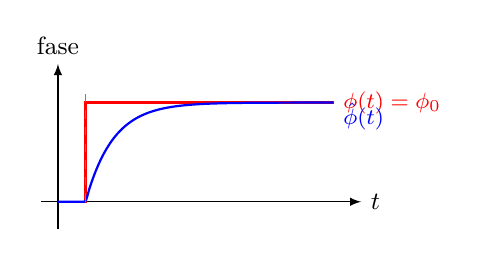
\begin{tikzpicture}[>=latex, scale=0.7]
\draw[->] (-0.3,0) -- (5.5,0) node[right, font=\small] {$t$};
\draw[->] (0,-0.5) -- (0,2.5) node[above, font=\small] {fase};
% Fase real (degrau)
\draw[thick, red] (0,0) -- (0.5,0) -- (0.5,1.8) -- (5,1.8);
\node[right, font=\footnotesize, red] at (5,1.8) {$\phi(t) = \phi_0$};
% Estimativa PLL
\draw[thick, blue, smooth] plot[domain=0:5, samples=80]
  (\x, {ifthenelse(\x<0.5, 0, 1.8*(1-exp(-2*(\x-0.5))))});
\node[right, font=\footnotesize, blue] at (5,1.55) {$\hat{\phi}(t)$};
\draw[dashed, gray] (0.5,0) -- (0.5,2);
\end{tikzpicture}
\end{center}
\end{column}
\begin{column}{0.48\textwidth}
\begin{center}
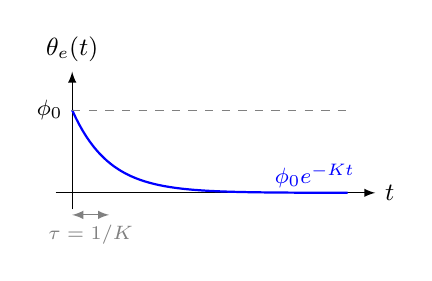
\begin{tikzpicture}[>=latex, scale=0.7]
\draw[->] (-0.3,0) -- (5.5,0) node[right, font=\small] {$t$};
\draw[->] (0,-0.3) -- (0,2.2) node[above, font=\small] {$\theta_e(t)$};
\draw[thick, blue] plot[domain=0:5, samples=80] (\x, {1.5*exp(-1.5*\x)});
\node[blue, font=\footnotesize, right] at (3.5,0.3) {$\phi_0 e^{-Kt}$};
\draw[dashed, gray] (0,1.5) -- (5,1.5);
\node[left, font=\footnotesize] at (0,1.5) {$\phi_0$};
\draw[<->, gray] (0.67,-0.4) -- node[below, font=\scriptsize] {$\tau = 1/K$} (0,-0.4);
\end{tikzpicture}
\end{center}
\end{column}
\end{columns}

\vspace{0.2cm}

Para PLL de 2ª ordem ($F(s) = 1 + a/s$): o resultado é o mesmo ($\theta_e \to 0$), mas com convergência mais rápida. Ambas as ordens \textbf{eliminam} o erro para degrau.
}

\only<8>{
\textbf{Perturbação 2: Rampa de fase / Doppler} --- PLL de 1ª ordem

\vspace{0.15cm}

\textbf{Passo 1:} Definir a entrada e sua transformada.
\[
\phi(t) = \Delta\omega\,t \quad\xrightarrow{\;\mathcal{L}\;}\quad \Phi(s) = \frac{\Delta\omega}{s^2}
\]

\vspace{0.1cm}

\textbf{Passo 2:} Substituir na expressão do erro.
\[
\Theta_e(s) = \frac{\Delta\omega}{s^2}\cdot\frac{s}{s+K} = \frac{\Delta\omega}{s(s+K)}
\]

\vspace{0.1cm}

\textbf{Passo 3:} Frações parciais.
\[
\frac{\Delta\omega}{s(s+K)} = \frac{\Delta\omega}{K}\left(\frac{1}{s} - \frac{1}{s+K}\right)
\]
}

\only<9>{
\textbf{Perturbação 2: Rampa de fase / Doppler} --- regime permanente

\vspace{0.15cm}

\textbf{Passo 4:} Voltar ao tempo.
\[
\boxed{\theta_e(t) = \frac{\Delta\omega}{K}\left(1 - e^{-Kt}\right), \quad t \geq 0}
\]

\vspace{0.2cm}

\textbf{Passo 5:} Valor em regime permanente.
\[
\theta_e(\infty) = \frac{\Delta\omega}{K}(1 - 0) = \boxed{\frac{\Delta\omega}{K}}
\]

\vspace{0.2cm}

O erro não vai a zero: o PLL de 1ª ordem segue a rampa com um atraso de fase constante,
tanto menor quanto maior o ganho $K$ do laço.
}

\only<10>{
\textbf{Perturbação 2: Rampa} --- PLL de 2ª ordem

\vspace{0.1cm}

Com $F(s) = 1 + \frac{a}{s}$, a função de transferência de erro muda:
\vspace{-0.15cm}
\[
1-H(s) = \frac{s^2}{s^2 + Ks + Ka}
\]

\vspace{-0.25cm}

Substituindo $\Phi(s) = \Delta\omega/s^2$:
\vspace{-0.15cm}
\[
\Theta_e(s) = \frac{\cancel{s^2}}{s^2 + Ks + Ka}\cdot\frac{\Delta\omega}{\cancel{s^2}} = \frac{\Delta\omega}{s^2 + Ks + Ka}
\]

\vspace{-0.25cm}

Pelo teorema do valor final:
\vspace{-0.15cm}
\[
\theta_e(\infty) = \lim_{s\to 0}\, s\cdot\frac{\Delta\omega}{s^2 + Ks + Ka} = \frac{0}{Ka} = \boxed{0}
\]

\vspace{-0.1cm}

O integrador no filtro $F(s)$ \textbf{elimina} o erro para rampa: o PLL de 2ª ordem rastreia
perfeitamente um desvio Doppler constante.
}

\only<11>{
\textbf{Resumo: erro em regime permanente}

\vspace{0.3cm}

\begin{center}
\begin{tabular}{l c c}
\hline
\textbf{Perturbação} & \textbf{PLL 1ª ordem} & \textbf{PLL 2ª ordem} \\
\hline
Degrau de fase ($\phi_0$) & $\theta_e \to 0$ & $\theta_e \to 0$ \\[4pt]
Rampa / Doppler ($\Delta\omega\,t$) & $\theta_e = \dfrac{\Delta\omega}{K}$ & $\theta_e \to 0$ \\
\hline
\end{tabular}
\end{center}

\vspace{0.3cm}

Para manter $|\theta_e| < 30°$ com PLL de 1ª ordem: basta $K$ suficientemente grande.

\vspace{0.3cm}

\colorbox{orange!12}{\parbox{0.9\textwidth}{\small\centering
\textbf{Atenção:} A aproximação é \textit{autoconsistente} --- se o PLL está travado e o ganho $K$ é adequado, $\theta_e$ permanece pequeno, validando a própria análise linear que usamos para projetá-lo.
}}
}

\end{frame}

% ============================================
% SLIDE: Como o PLL estima a fase
% ============================================
\begin{frame}{Como o PLL Estima a Fase}

\only<2>{
\textbf{Dinâmica do travamento:}

\begin{center}
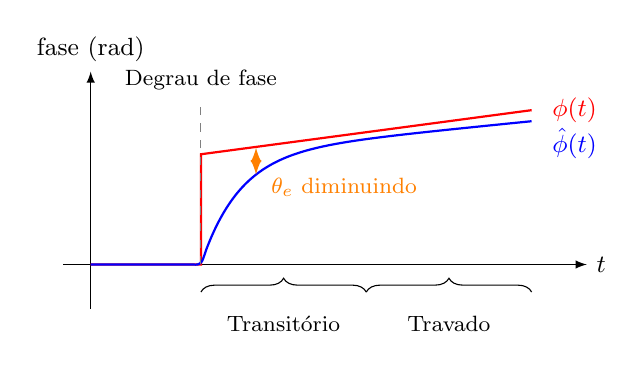
\begin{tikzpicture}[>=latex, scale=0.7]
\draw[->] (-0.5,0) -- (9,0) node[right, font=\small] {$t$};
\draw[->] (0,-0.8) -- (0,3.5) node[above, font=\small] {fase (rad)};

% Fase real (degrau + drift)
\draw[thick, red] (0,0) -- (2,0) -- (2,2) -- (8,2.8);
\node[right, font=\small, red] at (8.2,2.8) {$\phi(t)$};

% Estimativa PLL
\draw[thick, blue, smooth] plot[domain=0:8, samples=100]
  (\x, {ifthenelse(\x<2, 0,
        2*(1-exp(-1.5*(\x-2))) + 0.1*(\x-2) * (1-exp(-1.5*(\x-2))))});
\node[right, font=\small, blue] at (8.2,2.2) {$\hat{\phi}(t)$};

% Marca do degrau
\draw[dashed, gray] (2,0) -- (2,3);
\node[above, font=\footnotesize] at (2,3) {Degrau de fase};

% Erro
\draw[<->, thick, orange] (3,2.12) -- (3,{2*(1-exp(-1.5))+ 0.1*(1-exp(-1.5))});
\node[right, font=\footnotesize, orange] at (3.1,1.4) {$\theta_e$ diminuindo};

% Regiões
\draw[decorate, decoration={brace, amplitude=5pt}] (2,-0.5) -- (5,-0.5)
  node[midway, below=5pt, font=\footnotesize] {Transitório};
\draw[decorate, decoration={brace, amplitude=5pt}] (5,-0.5) -- (8,-0.5)
  node[midway, below=5pt, font=\footnotesize] {Travado};
\end{tikzpicture}
\end{center}

\vspace{-0.2cm}
PLL detecta erro $\theta_e$ $\rightarrow$ ajusta VCO $\rightarrow$ $\hat{\phi}(t)$ converge para $\phi(t)$
}

\only<1>{
\textbf{Parâmetros importantes do PLL:}

\vspace{0.3cm}

\begin{center}
\begin{tabular}{l l}
\textbf{Parâmetro} & \textbf{Significado} \\
\hline
$K = K_d K_v$ & Ganho de malha \\
$\omega_n$ & Frequência natural \\
$\zeta$ & Fator de amortecimento \\
$\Delta f_{\text{lock}}$ & Faixa de travamento \\
$\Delta f_{\text{capture}}$ & Faixa de captura \\
\end{tabular}
\end{center}

\vspace{0.3cm}

\textbf{Trade-off fundamental:}

\begin{columns}[T]
\begin{column}{0.48\textwidth}
\textbf{$K$ grande:}
\begin{itemize}
\item Rastreio rápido
\item Erro em regime pequeno
\item Mais ruído na saída
\end{itemize}
\end{column}
\begin{column}{0.48\textwidth}
\textbf{$K$ pequeno:}
\begin{itemize}
\item Rastreio lento
\item Mais robusto ao ruído
\item Erro em regime maior
\end{itemize}
\end{column}
\end{columns}
}

\end{frame}

% ============================================
% SLIDE: PLL em ação
% ============================================
\begin{frame}{PLL em Ação: Recuperação de Portadora}

\begin{center}
\includegraphics[width=\figFull]{figures/cap4/pll_recovery.pdf}
\end{center}

\vspace{-0.2cm}
O PLL converge rapidamente e o sinal recuperado acompanha o original

\end{frame}

% ============================================
% SLIDE: Sem PLL — perda de sincronismo
% ============================================
\begin{frame}{Sem PLL: Efeito do Erro de Fase}

\begin{center}
\includegraphics[width=\figFull]{figures/cap4/pll_vs_no_pll.pdf}
\end{center}

\end{frame}

% %%%%%%%%%%%%%%%%%%%%%%%%%%%%%%%%%%%%%%%%%%%%
% EXERCÍCIOS — AM DSB-SC (Sincronismo e PLL)
% %%%%%%%%%%%%%%%%%%%%%%%%%%%%%%%%%%%%%%%%%%%%

\subsection*{Exercícios: Sincronismo e PLL}

% ============================================
\begin{frame}{Exercício: Erro de Sincronismo e PLL}

\only<1>{
Um receptor DSB-SC opera com $f_c = 10\,\text{MHz}$ e oscilador local
a quartzo com estabilidade de $\pm 1\,\text{ppm}$.

\vspace{0.3cm}

\begin{enumerate}[a)]
\item Qual o desvio máximo de frequência do oscilador local?
\item Sem PLL, se o erro de fase acumula até $45^{\circ}$,
      qual a atenuação (em dB)?
\item Um PLL de 1ª ordem com $K = 2\pi \times 500$ rad/s é usado.
      Se o Doppler causa $\Delta\omega = 2\pi \times 50$ rad/s,
      qual o erro de fase em regime permanente?
\item Qual a atenuação com PLL? Compare com o item b).
\end{enumerate}
}

\only<2>{
\textbf{a)} $\Delta f = 1\,\text{ppm} \times 10\,\text{MHz} = \boxed{10\,\text{Hz}}$

\textbf{b)} $\cos 45^{\circ} = 0.707$ \quad $\rightarrow$ \quad $20\log_{10}(0.707) = \boxed{-3.0\,\text{dB}}$

\textbf{c)} $\theta_e(\infty) = \frac{\Delta\omega}{K} = \frac{2\pi \times 50}{2\pi \times 500} = \boxed{0.1\,\text{rad} = 5.7^{\circ}}$

\textbf{d)} $\cos(5.7^{\circ}) = 0.995$ \quad $\rightarrow$ \quad $20\log_{10}(0.995) = -0.04\,\text{dB}$

\vspace{0.3cm}

\begin{center}
\begin{tabular}{l c c}
 & \textbf{Sem PLL} & \textbf{Com PLL} \\
\hline
Erro de fase & $45^{\circ}$ & $5.7^{\circ}$ \\
Atenuação & $-3.0$ dB & $-0.04$ dB \\
\end{tabular}
\end{center}

O PLL reduz a perda de $-3$ dB para desprezível!
}

\end{frame}

% ============================================
\begin{frame}{Exercício: Dimensionamento do PLL}

\only<1>{
Um sistema de comunicação móvel usa DSB-SC em $f_c = 900\,\text{MHz}$.
O veículo se desloca a $v = 120\,\text{km/h}$.

\vspace{0.2cm}

\begin{enumerate}[a)]
\item Calcule o desvio Doppler $\Delta f$.
\item Qual deve ser o ganho mínimo $K$ do PLL para que o erro de fase
      em regime não exceda $5^{\circ}$?
\item Se o PLL tem $K = 2\pi \times 2000$ rad/s, qual o tempo de
      aquisição aproximado ($\tau \approx 1/K$)?
\item Um PLL de 2ª ordem seria melhor neste caso? Por quê?
\end{enumerate}
}

\only<2>{
\textbf{a) Calcule o desvio Doppler $\Delta f$.}

\vspace{0.3cm}

O efeito Doppler causa um desvio de frequência proporcional à velocidade relativa:
\[
\Delta f = \frac{v}{c}\,f_c
\]

\vspace{0.2cm}

Convertendo $v = 120\,\text{km/h} = \dfrac{120}{3{,}6} = 33{,}3\,\text{m/s}$:

\[
\Delta f = \frac{33{,}3}{3\times 10^8} \times 900\times 10^6 = \boxed{100\,\text{Hz}}
\]

\vspace{0.2cm}

Isso equivale a $\Delta\omega = 2\pi \times 100\,\text{rad/s}$.
}

\only<3>{
\textbf{b) Ganho mínimo $K$ para erro $\leq 5°$.}

\vspace{0.3cm}

O Doppler é uma rampa de fase. Para PLL de 1ª ordem, o erro em regime é:
\[
\theta_e(\infty) = \frac{\Delta\omega}{K}
\]

Queremos $\theta_e \leq 5° = 0{,}087\,\text{rad}$:
\[
\frac{\Delta\omega}{K} \leq 0{,}087
\quad\Rightarrow\quad
K \geq \frac{\Delta\omega}{0{,}087} = \frac{2\pi \times 100}{0{,}087}
\]
\[
\boxed{K \geq 2\pi \times 1149\,\text{rad/s}}
\]
}

\only<4>{
\textbf{c) Tempo de aquisição para $K = 2\pi \times 2000\,\text{rad/s}$.}

\vspace{0.3cm}

Para PLL de 1ª ordem, a constante de tempo é:
\[
\tau = \frac{1}{K}
\]

\vspace{0.1cm}

\[
\tau = \frac{1}{2\pi \times 2000} = \boxed{0{,}08\,\text{ms}}
\]

\vspace{0.3cm}

A aquisição é rápida frente à escala de tempo da mensagem de áudio, cujo período
característico é da ordem de milissegundos.
}

\only<5>{
\textbf{d) Um PLL de 2ª ordem seria melhor?}

\vspace{0.3cm}

Sim. O PLL de 2ª ordem tem erro \textbf{zero} para rampa de fase:
\[
\theta_e(\infty) = 0 \quad\text{para Doppler constante}
\]

\vspace{0.2cm}

O de 1ª ordem sempre terá erro residual $\Delta\omega/K$, que só pode ser reduzido
aumentando $K$ --- mas $K$ grande demais alarga a banda do laço e amplifica ruído.
}

\end{frame}

% ============================================

